%----------------------------------------------------------------------------
\chapter{Részletes megvalósítás}
\label{sec:Details}
%----------------------------------------------------------------------------

Ebben a fejezetben a korábban röviden bemutatott építőelemekről adok egy részletsebb leírást.
Bemutatom, hogy az én projektemben milyen megoldásokat valósítottam meg a használatukkal.
Ahol van értelme diagramokon keresztül mutatom be a működését, ami látványos azt képekkel is illsóusztrálom.
Több kódrészet is szerepelni fog a fejezetben amiknek célja a kód működésének jobb mégétése.

\section{Compose}
\label{sec:Compose}

A Composeról korában már adtam egy átfogó leírást a \refstruc{sec:JetpackCompose}ban, most ebben a részben részleesebben bemutatom az alapaeleveket, használtatát és a keletekező képernyőket.

\subsection{Compose alapelvek, használata valós környezeteben}

Mivel a Compose egy deklreatív UI kit ezért összefoglalnám a legfontosabb részeit.
A UI elmeket nem lehet lehet direktben példányosítani, és kódból később elérni és ezen a referncián eresztül módosítani a tulajdonságait.
Minden egyes elem egy függvényhívást jelent, az állapotát és tulajdonságait pedig ezen belül lehet szábályozni és bállítani egyéb objektumokon és stateken keresztül.
Ezeket az állapotokat általában nem a Composable függvéyne belül tároljuk hanem egy ViewModelben, mivel az tartósabb. (\refstruc{fig:ViewModel})
Egy figyelt állapot hatására meghívódik a recomposoition, azaz a függvény újra meghívódik és frissíti a UI állapotát.
Az általános elv az, hogy egy Composable függvény nagy betűvel kezdődik, és attól lesz egy függvéyn Composable, hogy elé helyezzük a @Composable anntotációt.

Mi is az a recomposoition?
Röviden valamilyen állapotváltozást követő újra kirajzolódás.
Gyakran valamilyen felhasználói interakció váltja ki (gomb megnyomása, görgetés), de a ViewModelből is jöhet ez a változás (megérkezik a kezdeti adat, folyamotson frissülő információk jönnek), de okozhatja egy animáció is.

A Compose hasznátának van 5 fontos alapszáblya amelyek betartásával nem csak helyes, de gyors és dinamikus frissülő képernyőket tudunk egyszerűen létrehozni.
\begin{enumerate}
    \item A Composable függvények bármilyen sorrendben végrehajthatók.
    \item A Composable függvények párhuzamosan hajthatók végre.
    \item A Recomposition kihagyja a lehető legtöbb Composable függvényt és lambdát.
    \item A Recomposition optimista, és leállítható menet közben.
    \item Egy Composable függvény nagyon gyakran is futhat/ismétlődhet, olyan gyakran is, mint egy animáció minden képkockája.
\end{enumerate}

Pontosan mit is jelentenek ezek a szabályok?
Az 1. és 2. pont alapján következik, hogy minden Composable függvény önálló legyen, nem függhet egy másik Composable függvénytől sem.
Továbbá fontos, hogy ha ugyan azon stateet változtatják akkor az ne fusson le minden recomposoition során, ha ezt nem tartjuk be akkor folyamoatosn újra kirajzolódik a képernyő és lefagy az eszköz.
A 3. pont értelmezése, hogy csak a szükséges és részek renderelődnek újra, ezzel gyorsítva a folyamatot. Így amennyiben több függvényt is meghívnk egy másikon belül csak azok fognak újra rajzolódni amik függnek a változott állapottól.
Elő fordulhat, hogy mindent szeretnénk újra firissíteni, vagy több függvényt ami nem függ tőle, ehez használhatunk az állapottól függő Launched effectet vagy átadhatjuk az állaptot ezekenk a függvényknek is, és ott sinálhatumk vele egy egyszerű és gyors műveletet.
A 4. és 5. pont összefügg, ha új állapot érkezik és nem fejeződött be a recomposoition akkor előrről kedzi a folyamatot. Ne itt hajtsunk végre egy hosszú műveletet (HTTP kérések indítása), ez feleslges overheadet jelent mert senki nem állítja le az aszinkron hívást, és nem is tud hova visszaérkezni az adat így feleslgesen használtuk az erőforrsáokat mind a két oldalon.
Ne állítsunk be egy olyan értéet sem itt amire szükségünk lehet később, mivel nem biztos, hogy eljut a futás addig vagy, lehet, hogy a következő másodpercben már felül lett írva mással.

Az alábbi kódrészetben bemutatom, hogy milyen részekből tevődik össze egy Composable függvény.
\begin{lstlisting}[caption={Composable függvény részei.}, label={lst:ComposableParts}, language=Kotlin]
@Composable     // A kötelező annotáció
fun ExamEditResultScreen(   // Függvényparaméterek
    navigateBack: () -> Unit,       // Egy lambda függvény fejléce
    viewModel: ExamEditViewModel,   // ViewModel átadása paraméterként
    modifier: Modifier = Modifier   // Modifier amivel a kinézetet lehet testre szabdni.
) {
    val coroutineScope = rememberCoroutineScope()           // Coroutine scope lekérése, így lambda függényben használható, mivel annak a törzse nem Composable függvény.
    var showNotify by remember { mutableStateOf(false) }    // Statek amit el lehet tárolni a Composable függvényben mivel ezen kívül nincs használva.
    var notifyMessage by remember { mutableStateOf("") }    // Statek amit el lehet tárolni a Composable függvényben mivel ezen kívül nincs használva.
    if (showNotify) { Notify(notifyMessage); showNotify = false} // Állapottól függő megjelenítés
    Scaffold(   // Beépített Composable elem amivel egy általános Android nézetet könnyen létre lehet hozni.
        topBar = { TopAppBarContent(stringResource(Res.string.exam_edit), navigateBack) },  // Itt egy topBart lehet könnyen megadni.
    ){innerPadding ->   // Ez a belső része a képenyőnek, a fő része az alkalmazásnak.
        ExamEntryBody(      // Egy másik Composable elem meghívása, ami a megjelnésért felel.
            examUiState = viewModel.examUiState,           // Szüksége van viewModelben lévő statere
            onExamValueChange = viewModel::updateUiState,  // Nevesített függvényt így lehet átadni egy lambda függvénynek
            onSaveClick = {     // Lambda függvényt helyben is megadhatunk
                coroutineScope.launch { // Itt látható egy példa a trailing lambda használatára
                    if(viewModel.updateExam()){ navigateBack() }    // If-else szerkezet is nyugodtan használhatunk. Siker esetén visszanavigál
                    else{   // Egyéként a sikerttelenséget közli a felhasználóval
                        showNotify = true
                        notifyMessage =  "Exam with this name already exists"
                    }
                }
            },
            modifier = modifier.padding(innerPadding))}}
\end{lstlisting}

\subsection{Alkalmazás bemutatása képernyőképekkel}

Ebben az alfejezetben bemutatom az elkészült képernyőket és a hozzájuk tartozó érdekes részeket, megoldásokat.

\subsubsection{A fő képernyők}

A két alkalamzás típusra más-más a felhasználói igény.
Androidon, ahol általában egy álló képernyő van (\refstruc{fig:MainScreen} jobb oldal) és a telefont a jobb alsó sarokban fogjuk meg nem esik kézre a fent bekapcsolható menü (bár oldalra huzással is előhozható). 
Asztali alaklamzás estén viszont jobban mutat ez a megoláds, és egy nagyobb képernyő ahol a kiválasztott funkció képernyője meg tud jelenni. (\refstruc{fig:MainScreen} bal oldal és \refstruc{fig:OpenMenu})
Későbbiekben a mavigálásban is segít, így könnyebb képernyőt váltani, a fenti vissza gomb használata kevésbé kényelmes, mint Androidon egy gyos mozdulat a telefon alján, ahol a kenzünkkel tartjuk azt.

Ennek megfelelőn a MainScreen függvény a közös kódban egy expect függvény és így minden platformra az oda illő actual implementációt tudjuk megírni és alkalmazni.
Végül más megoldást váasztottam a navigációhoz, így az asztali alaklamzásnál a szintén expect/actual NavHost létrehozáskor nem kapnak értéket a függvények.
\begin{lstlisting}[caption={Expect Főképernyő.}, label={lst:ExpectMainScreen}, language=Kotlin]
@Composable
expect fun MainScreen(
    navigateToTopicList: () -> Unit = {},
    navigateToPointList: () -> Unit = {},
    navigateToTrueFalseQuestionList: () -> Unit = {},
    navigateToMultipleChoiceQuestionList: () -> Unit = {},
    navigateToExamList: () -> Unit = {},
    navigateToExportExamList: () -> Unit = {},
    navigateToSubmission: () -> Unit = {},
    onSignOut: () -> Unit = {},
)
\end{lstlisting}
\begin{figure}[!ht]
    \centering
    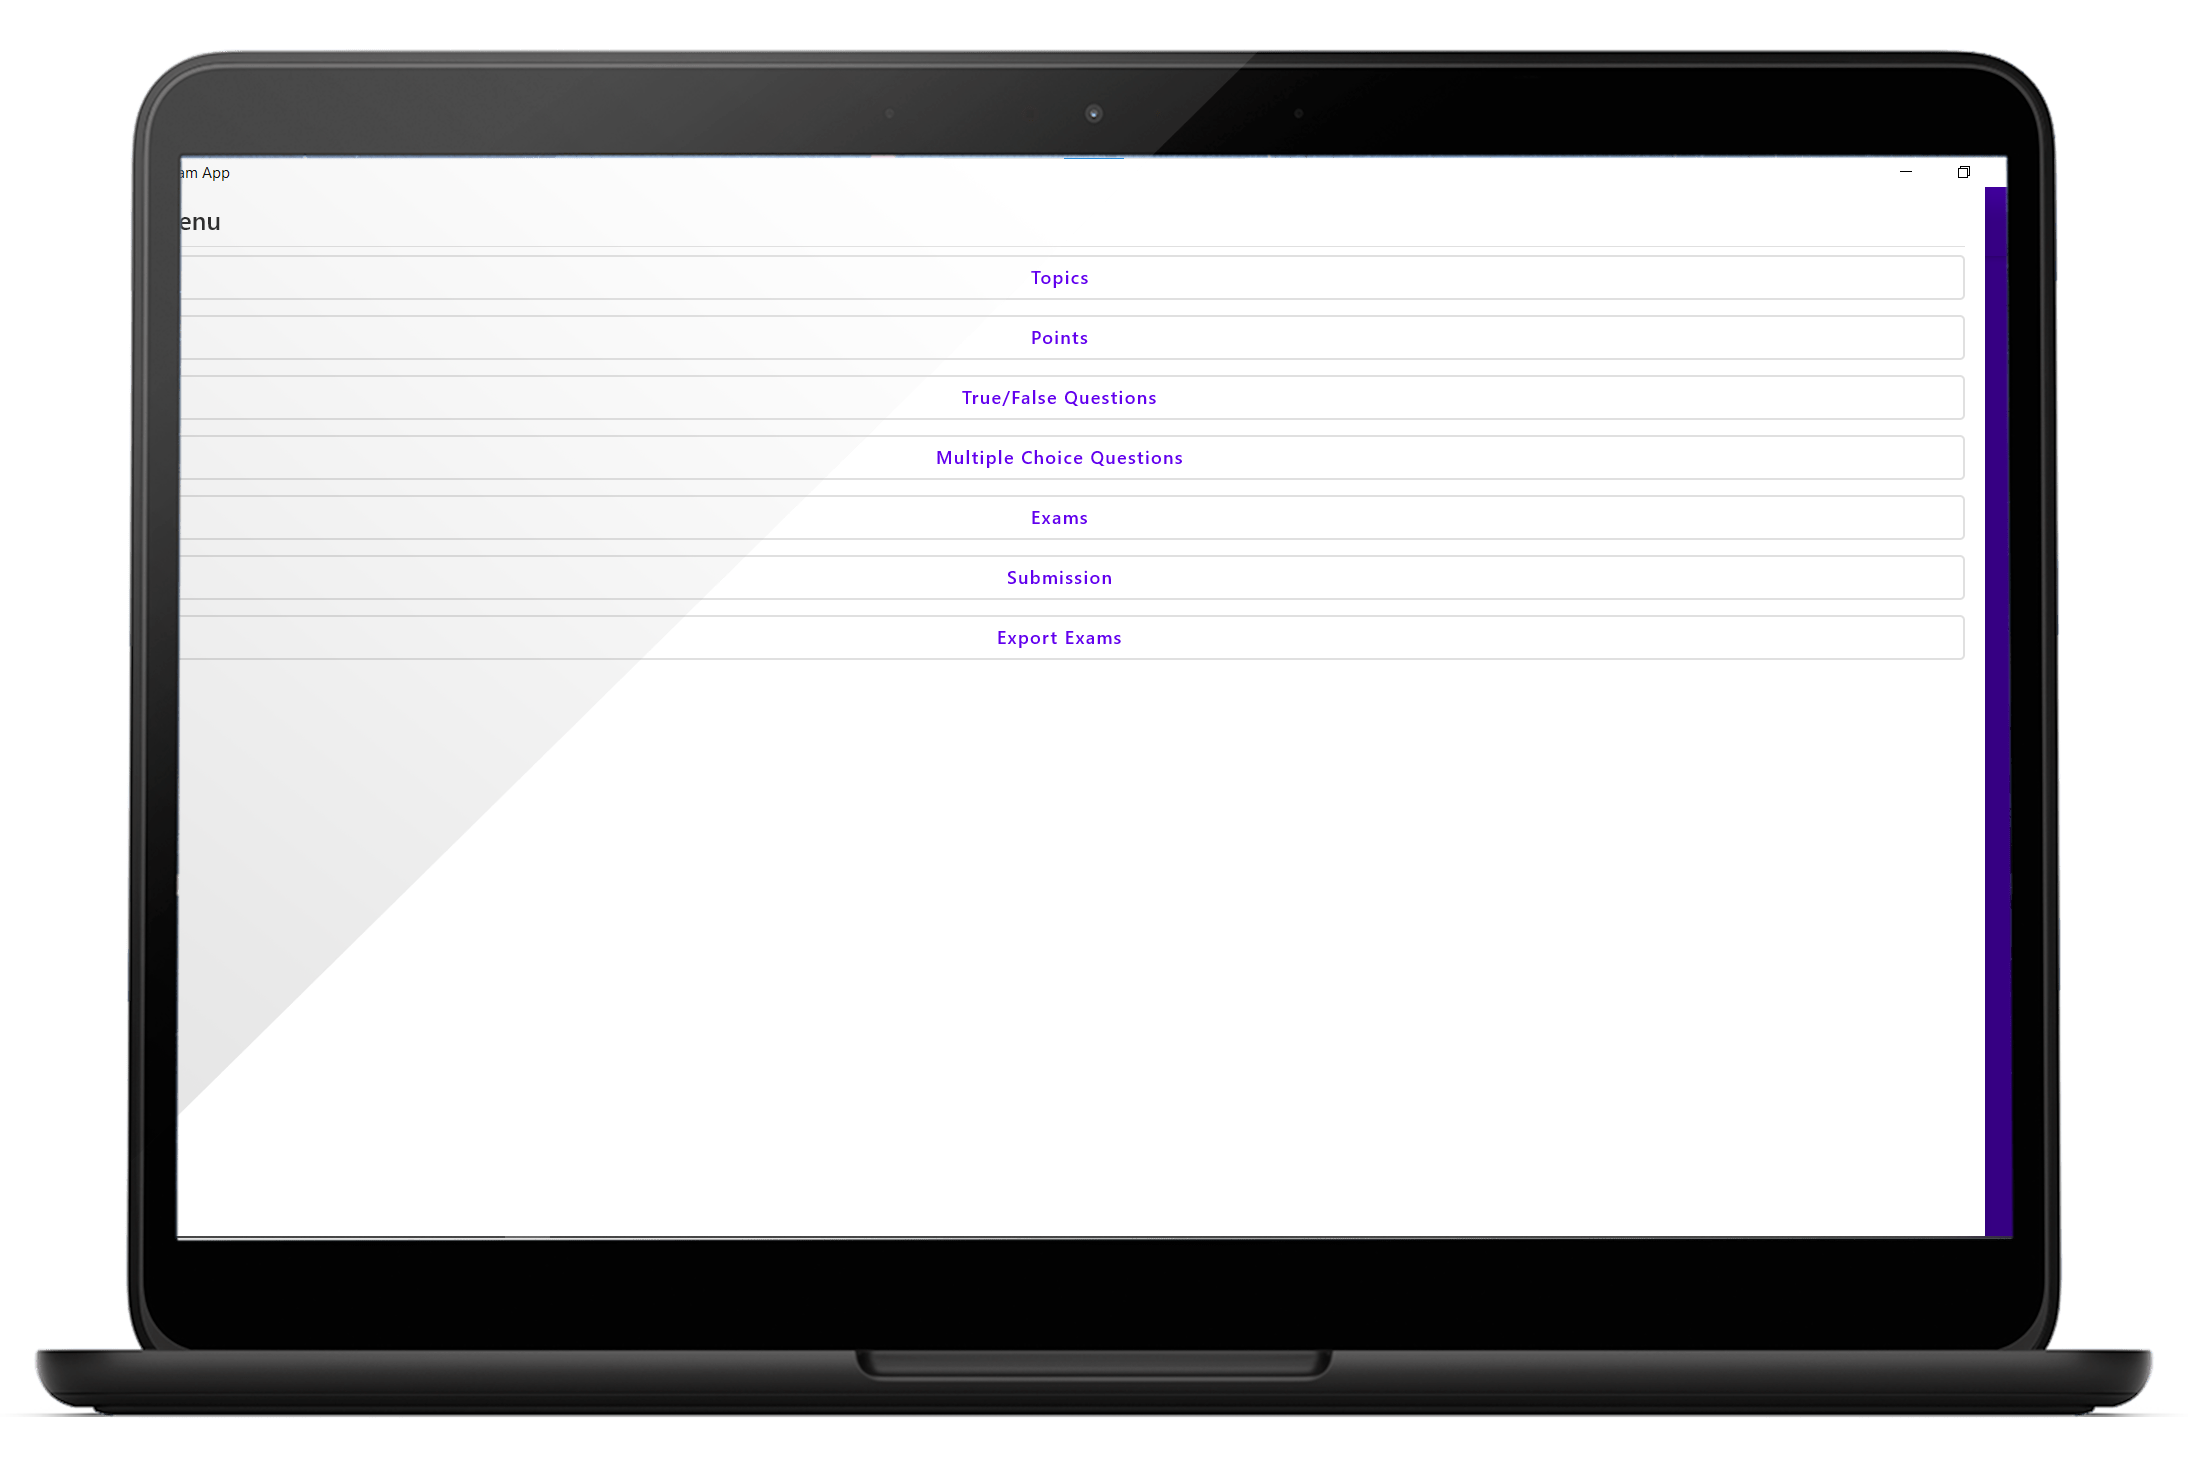
\includegraphics[width=0.5\textwidth, keepaspectratio]{figures/MainScreen_Desktop2_framed.png}
    \caption{Kinyitott menüsáv kinézete az asztali alkalmazáson}
    \label{fig:OpenMenu}
\end{figure}

\begin{figure}[!ht]
    \centering
    \begin{tabular}{cc}
        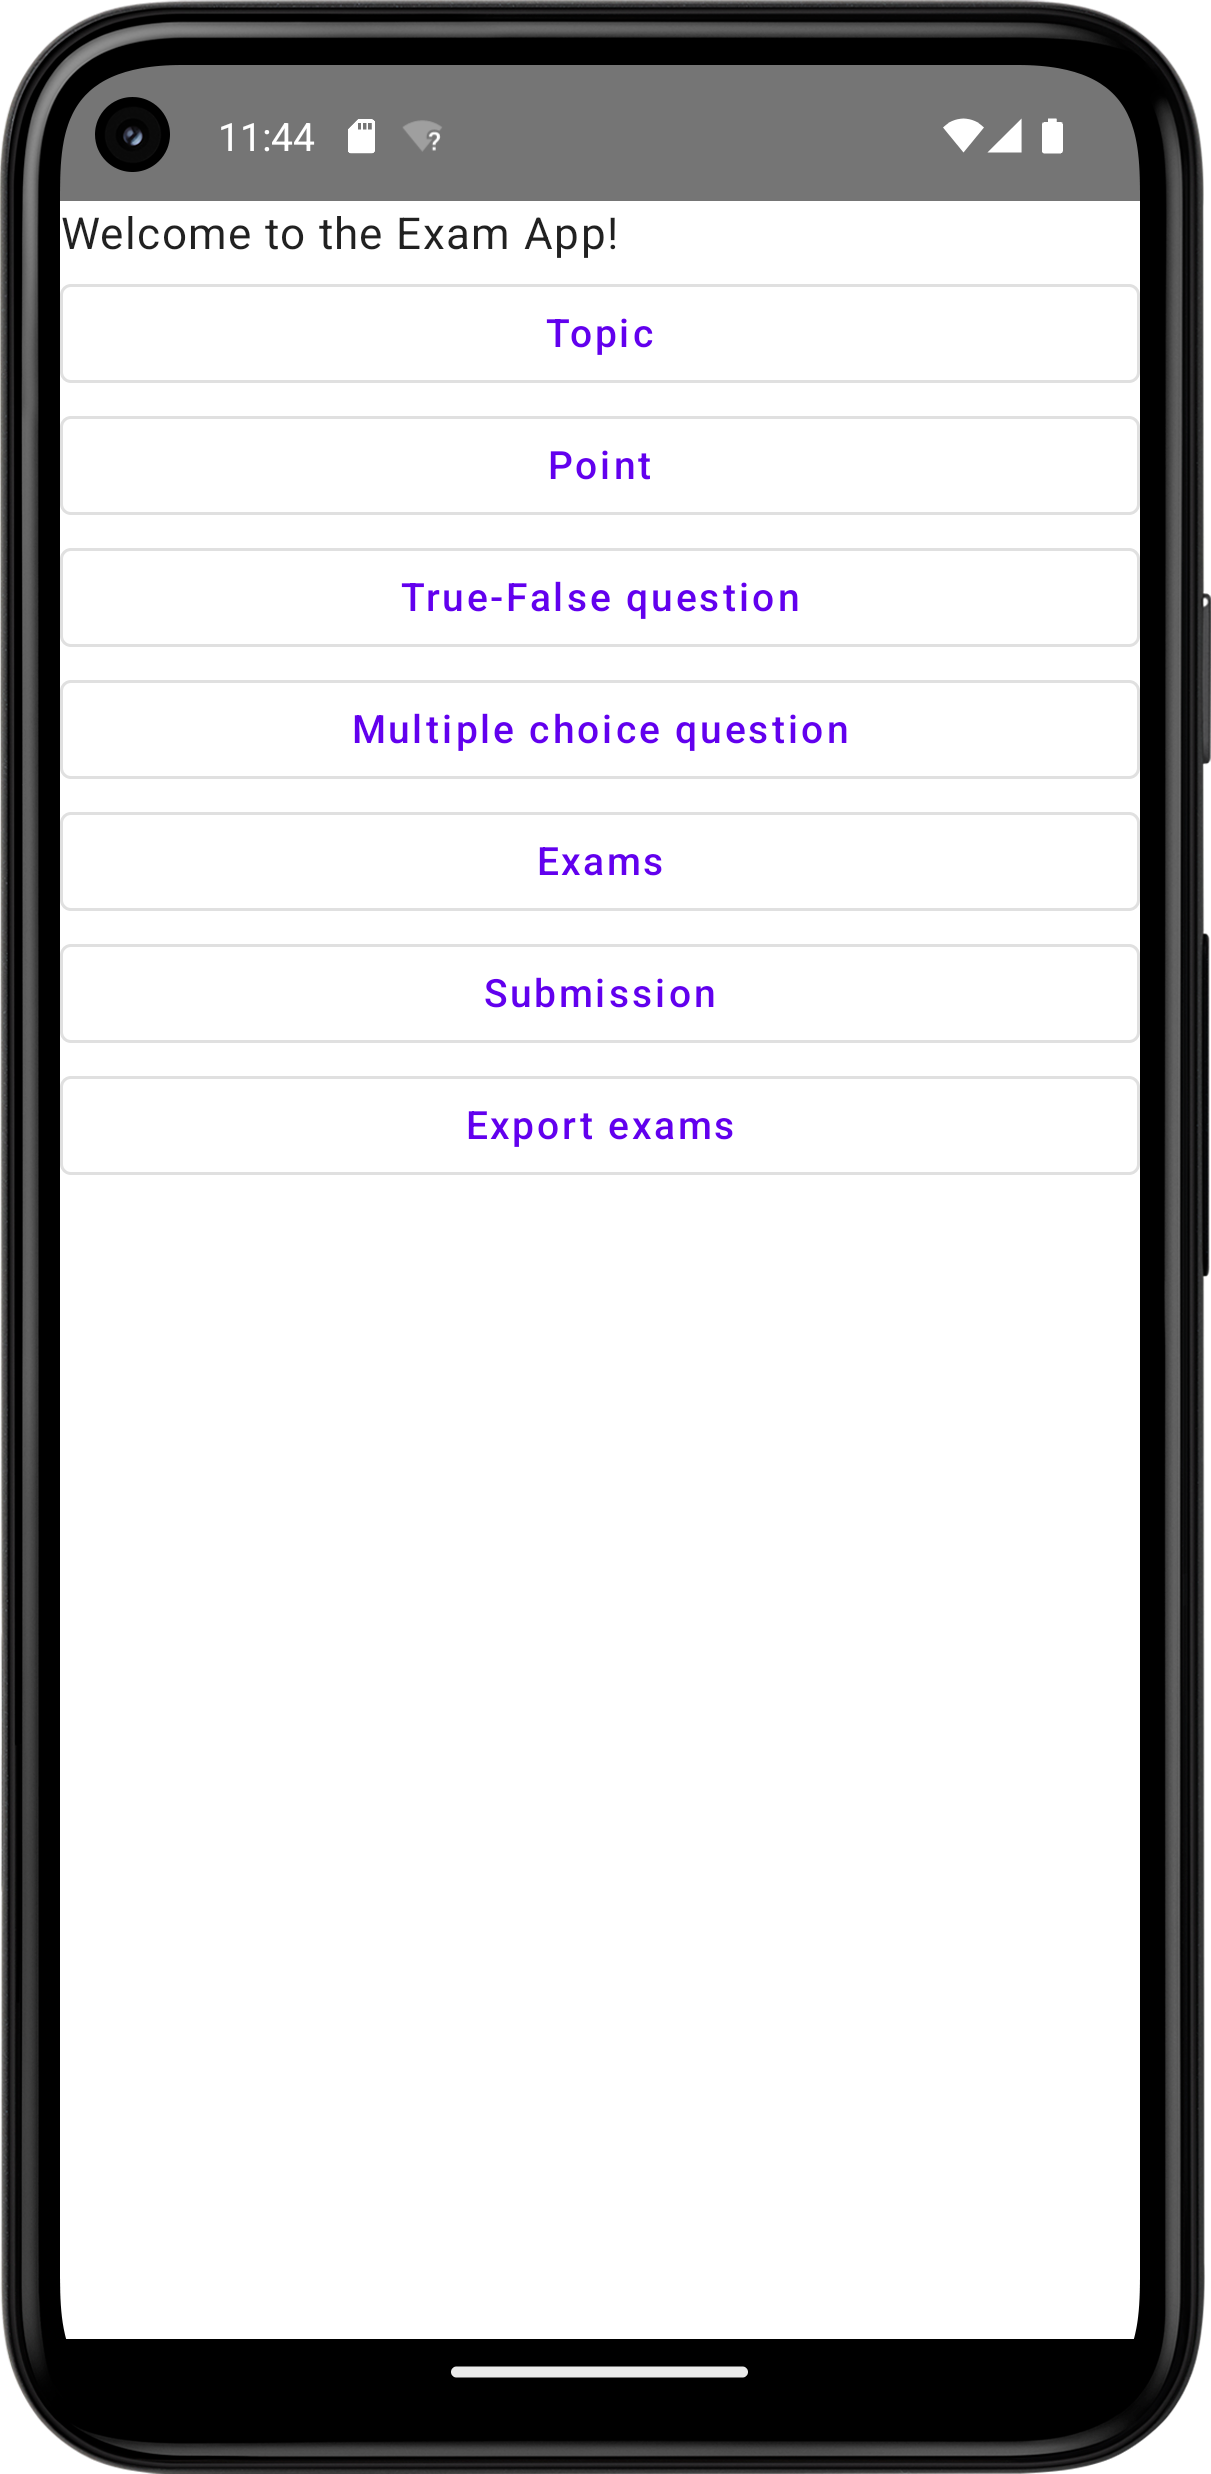
\includegraphics[width=0.3\textwidth, keepaspectratio]{figures/MainScreen_Android.png} & 
        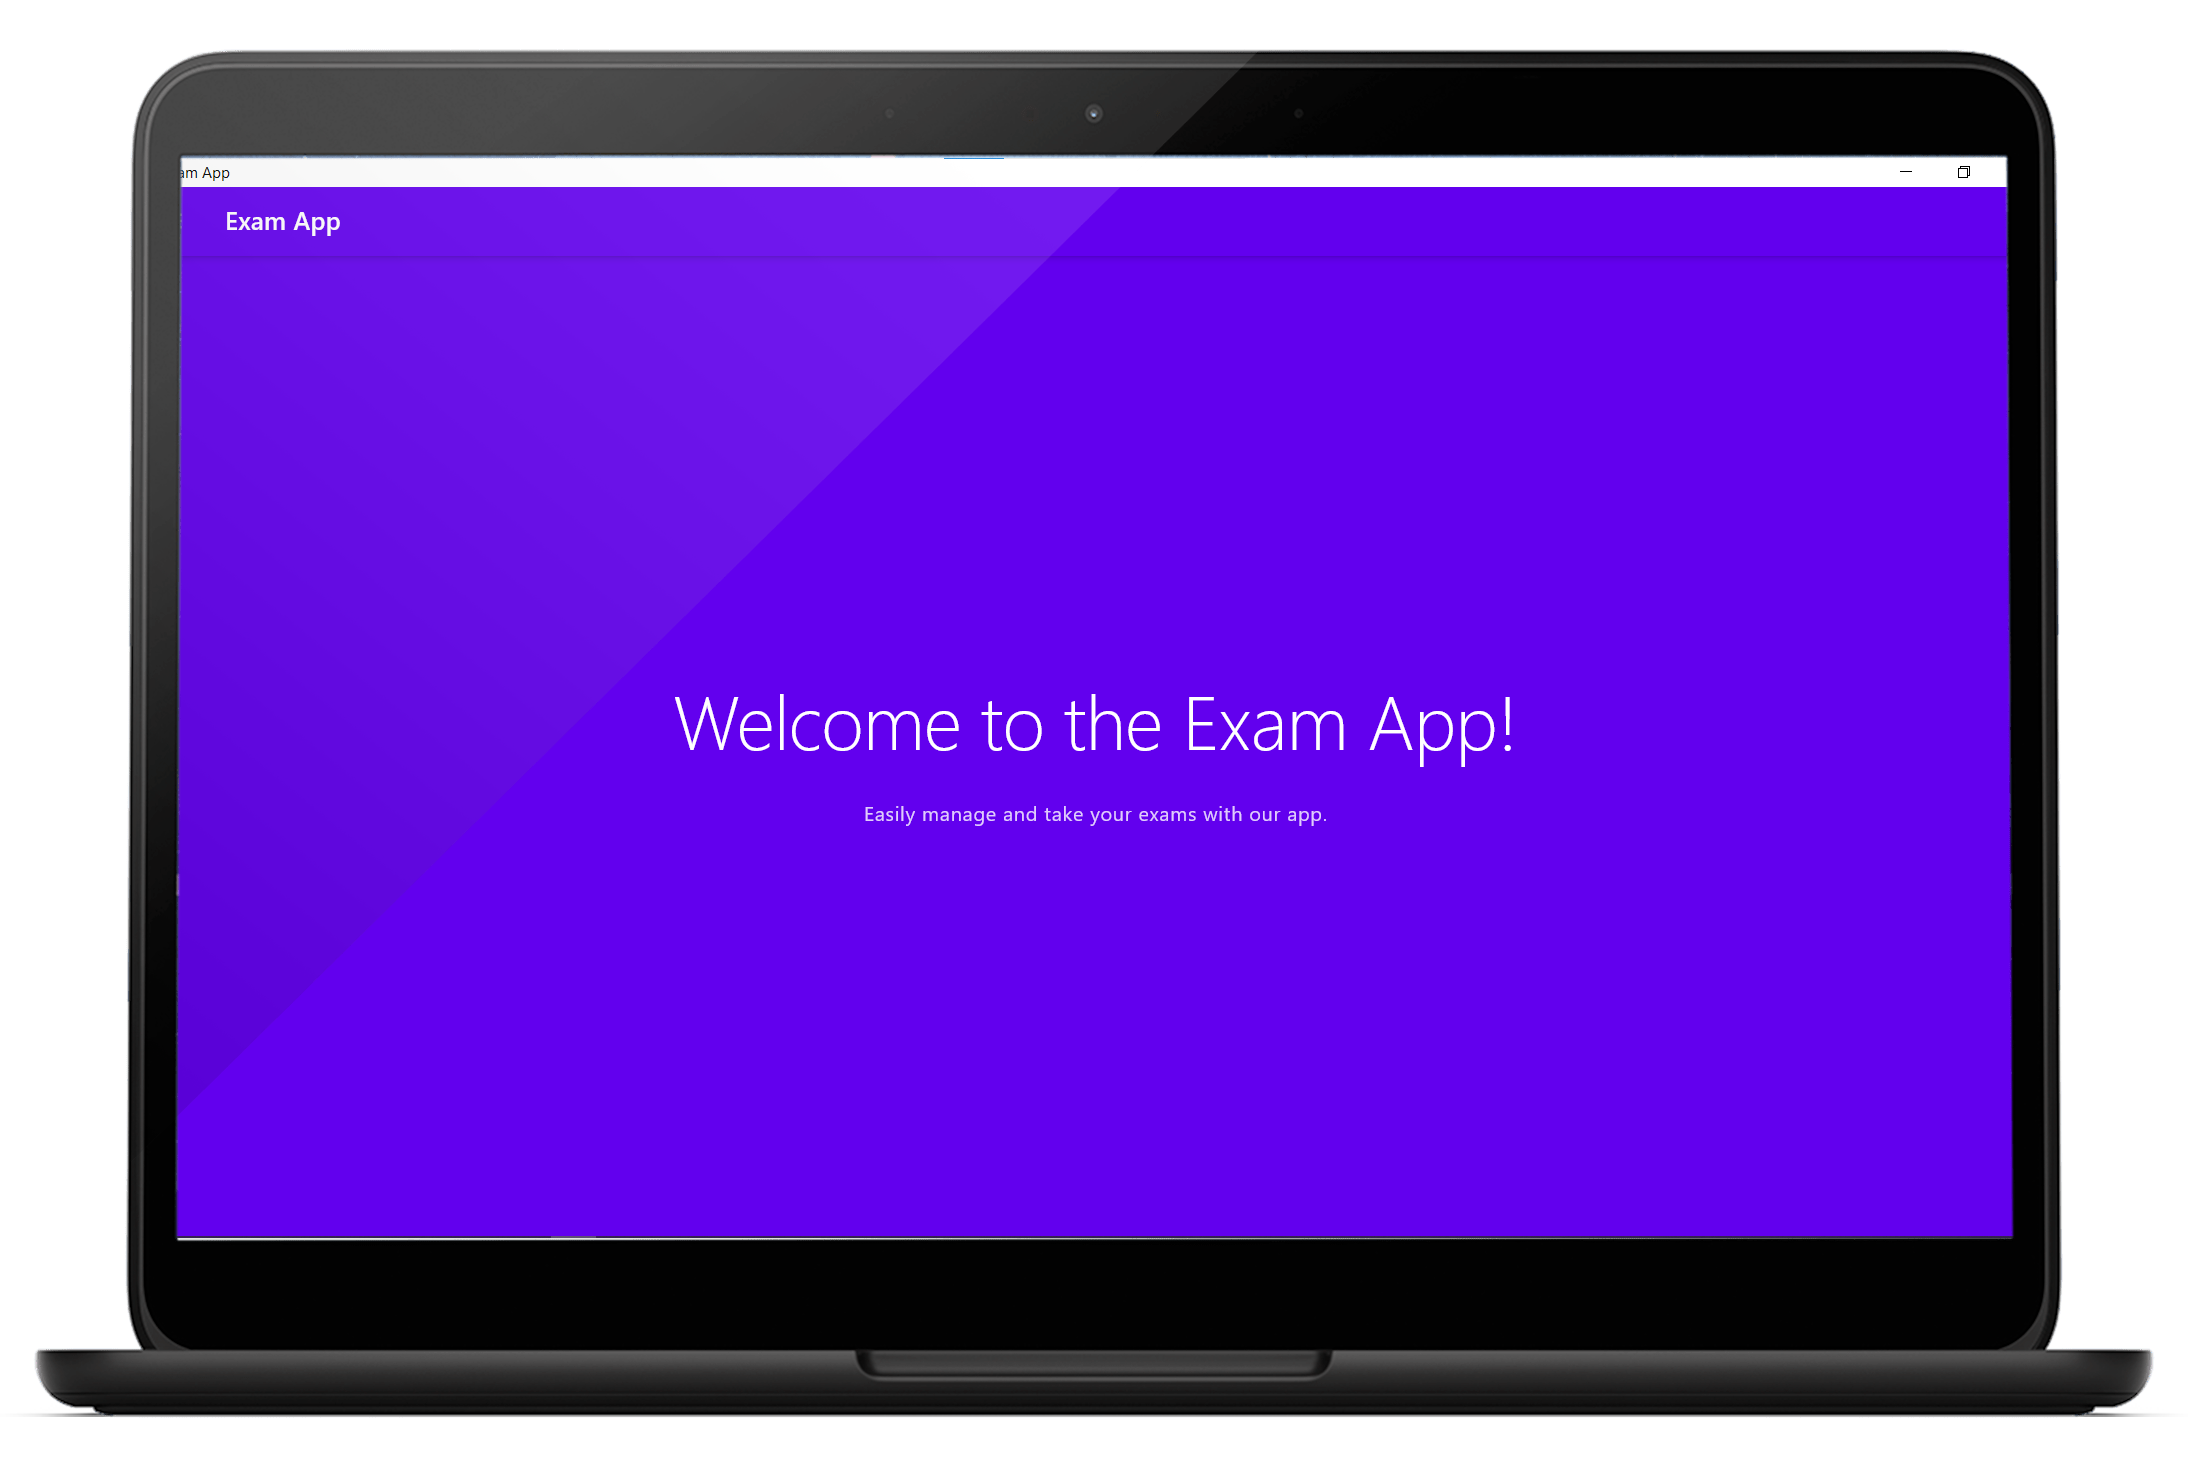
\includegraphics[width=0.5\textwidth, keepaspectratio]{figures/MainScreen_Desktop1_framed.png}
    \end{tabular}
    \caption{A fő képernyő Android és asztali alkalmazáson}
    \label{fig:MainScreen}
\end{figure}


\pagebreak

\subsubsection{Elemek listázása}

Az elemek felsorolásáért egy LazyColumn felel. (\ref{lst:ListScreen}.~kódrészet)
Ez egy előre létrehozott, beépített Composable függvéy.
Több hasznos tulajdonsággal rendelkezik. Alapértelmezett módon görgethetővé válik, ha több elem van benne, mint amennyi kifér egy képernyőre. (\refstruc{fig:ListScreen})
Alkalmas nagyon sok, akár végtelen elem megjelenítésére, bár ehhez szükség van az adtaok ügyes betöltésére is. 
Mindig csak annyi elemet renderel ki amennyi éppen szükséges, látszódik. Előtte és utána van egy kis tartalék puffer, így görgetés esetén nem kell várni az új adtaok betöltésére.
Az elemek testre is szabhatók benne, tökéltes alaklmaási területe lehet egy chat alkalmazás, ahol az elemeket az üzenet küldője alapján lehet színezni.

Ezen a képrenyőn is a Scaffold megoldást választottam így kényelemsen elfér egy navigációs sáv és egy Folating Action Button az új elemek felvételéhez.
Ezeken túl több korábban is bemutaott elem megjelenik ebben a kódrészletben is.
Ahogy látszik az alábbi kódrészetben is, attól függően lehet elemeket beállítani, hogy milyen feltételhet kötjöük az elemek megjelnítését.
\begin{lstlisting}[caption={Listázó képernyő.}, label={lst:ListScreen}, language=Kotlin]
@Composable
fun MultipleChoiceQuestionListResultScreen(
    ...
) {
    Scaffold(
        topBar = { TopAppBarContent(stringResource(Res.string.multiple_choice_question_list), navigateBack) },
        floatingActionButton = {
            FloatingActionButton(
                onClick = { addNewQuestion() }, ...
            ) {Icon(Icons.Filled.Add, contentDescription = "Add") }
        }
    ) { padding ->
        LazyColumn(
            contentPadding = padding,
            ...
        ) {
            if (questions.isEmpty()) {
                item { Box(modifier = Modifier ...) { Text(...) } }
            } else {
                items(questions) { question ->
                    TextButton(
                        onClick = { navigateToMultipleChoiceQuestionDetails(question.uuid) },
                        modifier = Modifier ...
                    ) {
                        Text(text = question.name, ...)
}}}}}}
\end{lstlisting}

\begin{figure}[!ht]
    \centering
    \begin{tabular}{cc}
        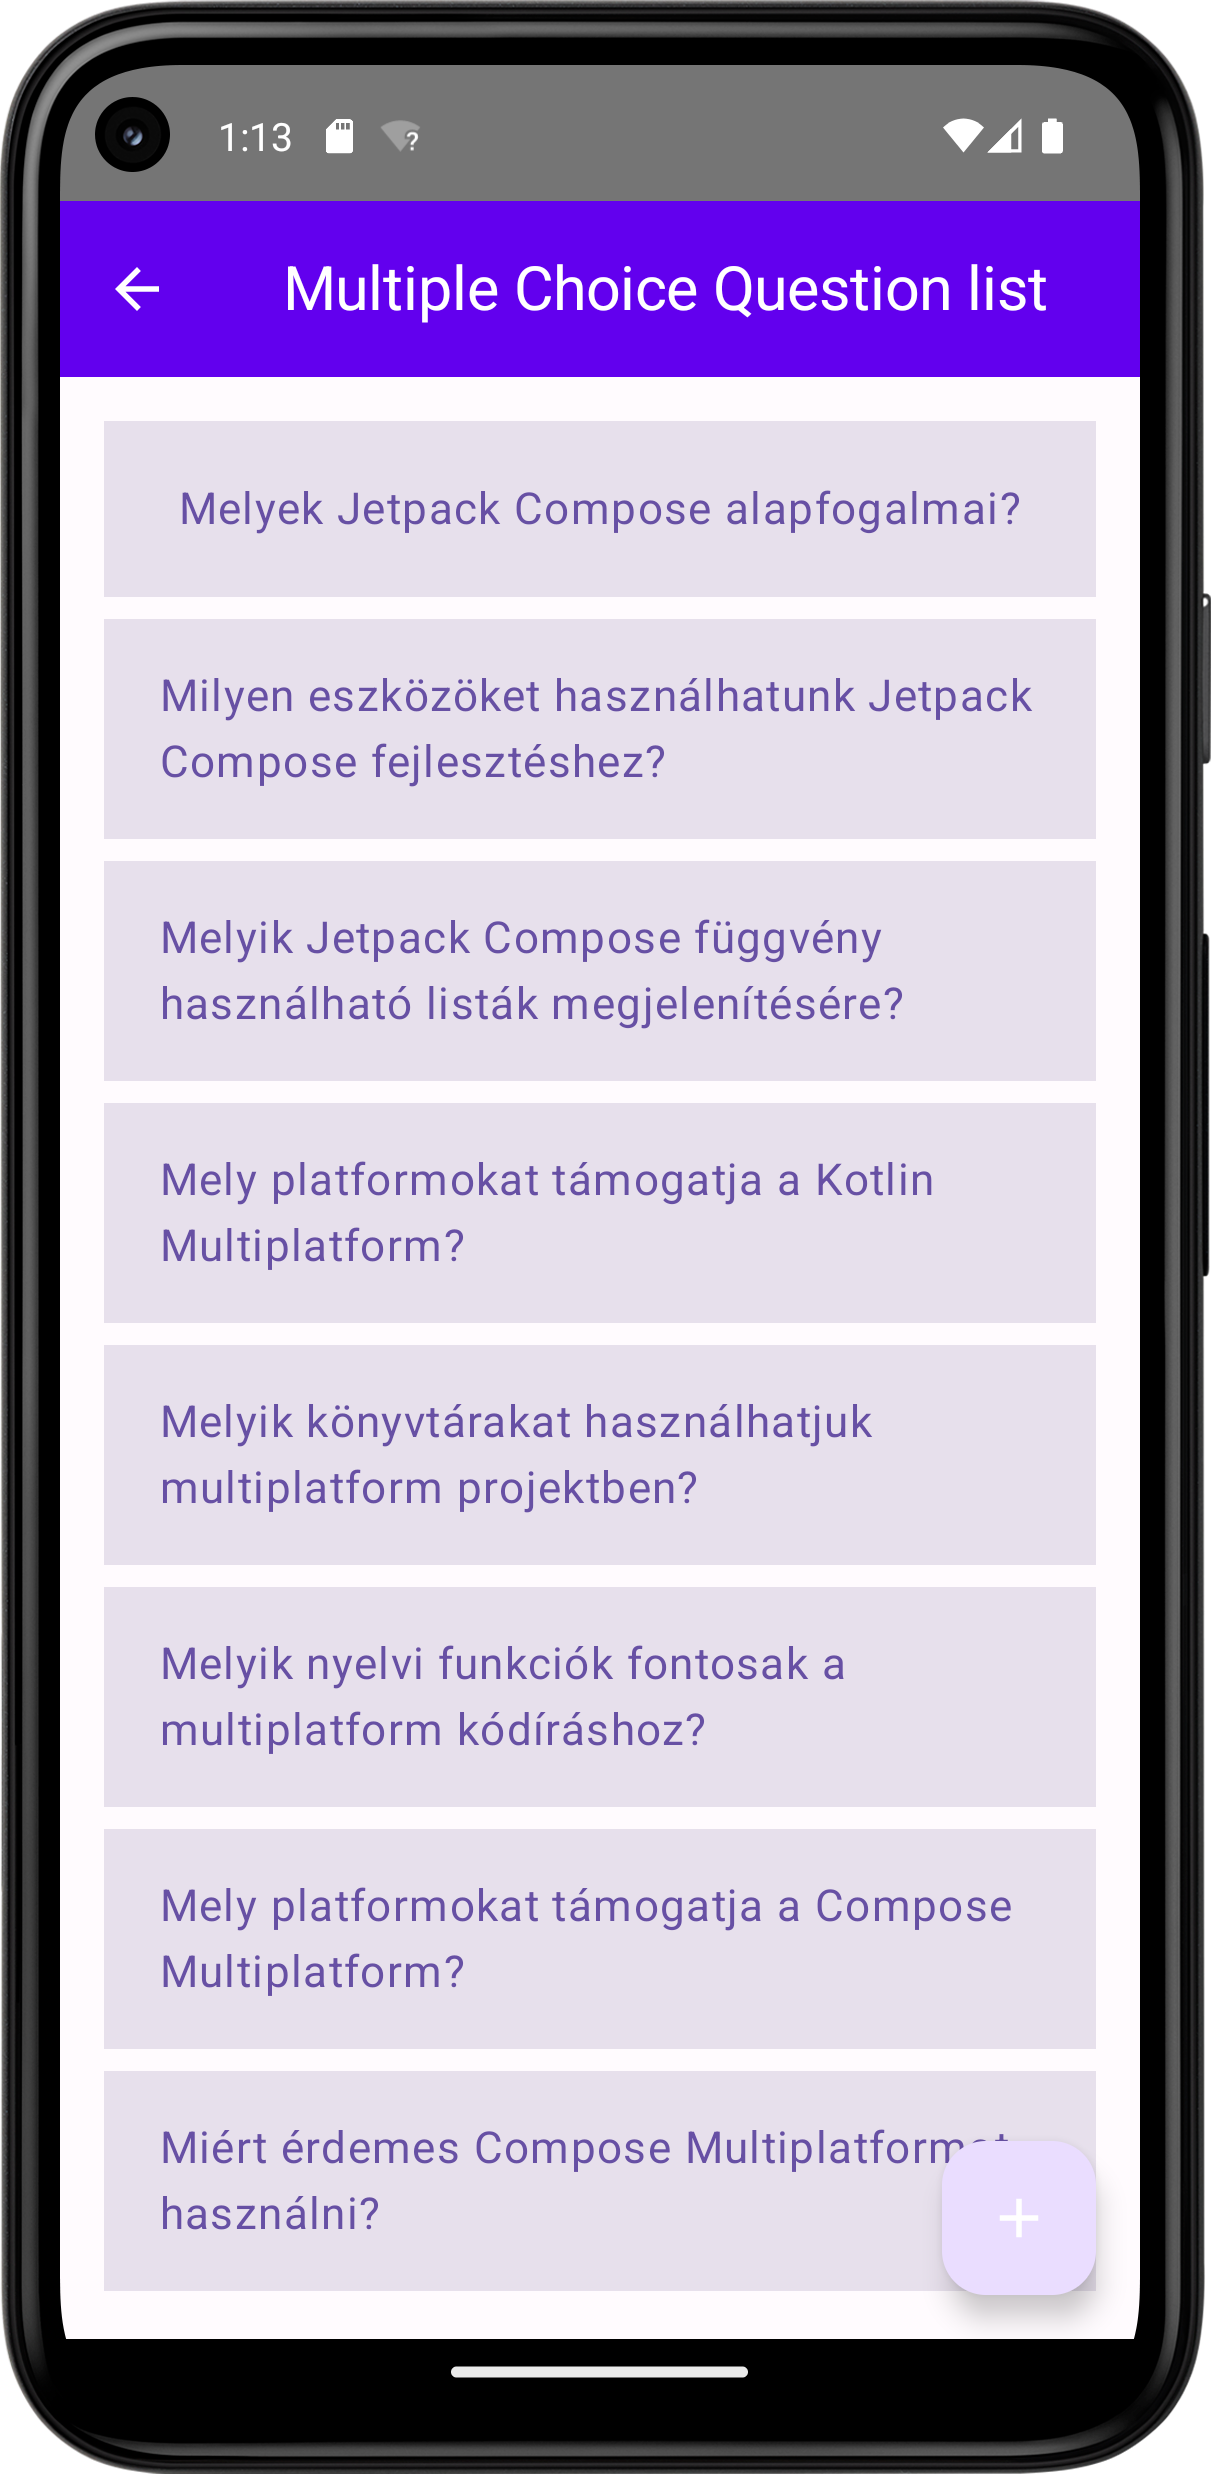
\includegraphics[width=0.3\textwidth, keepaspectratio]{figures/List_Android.png} & 
        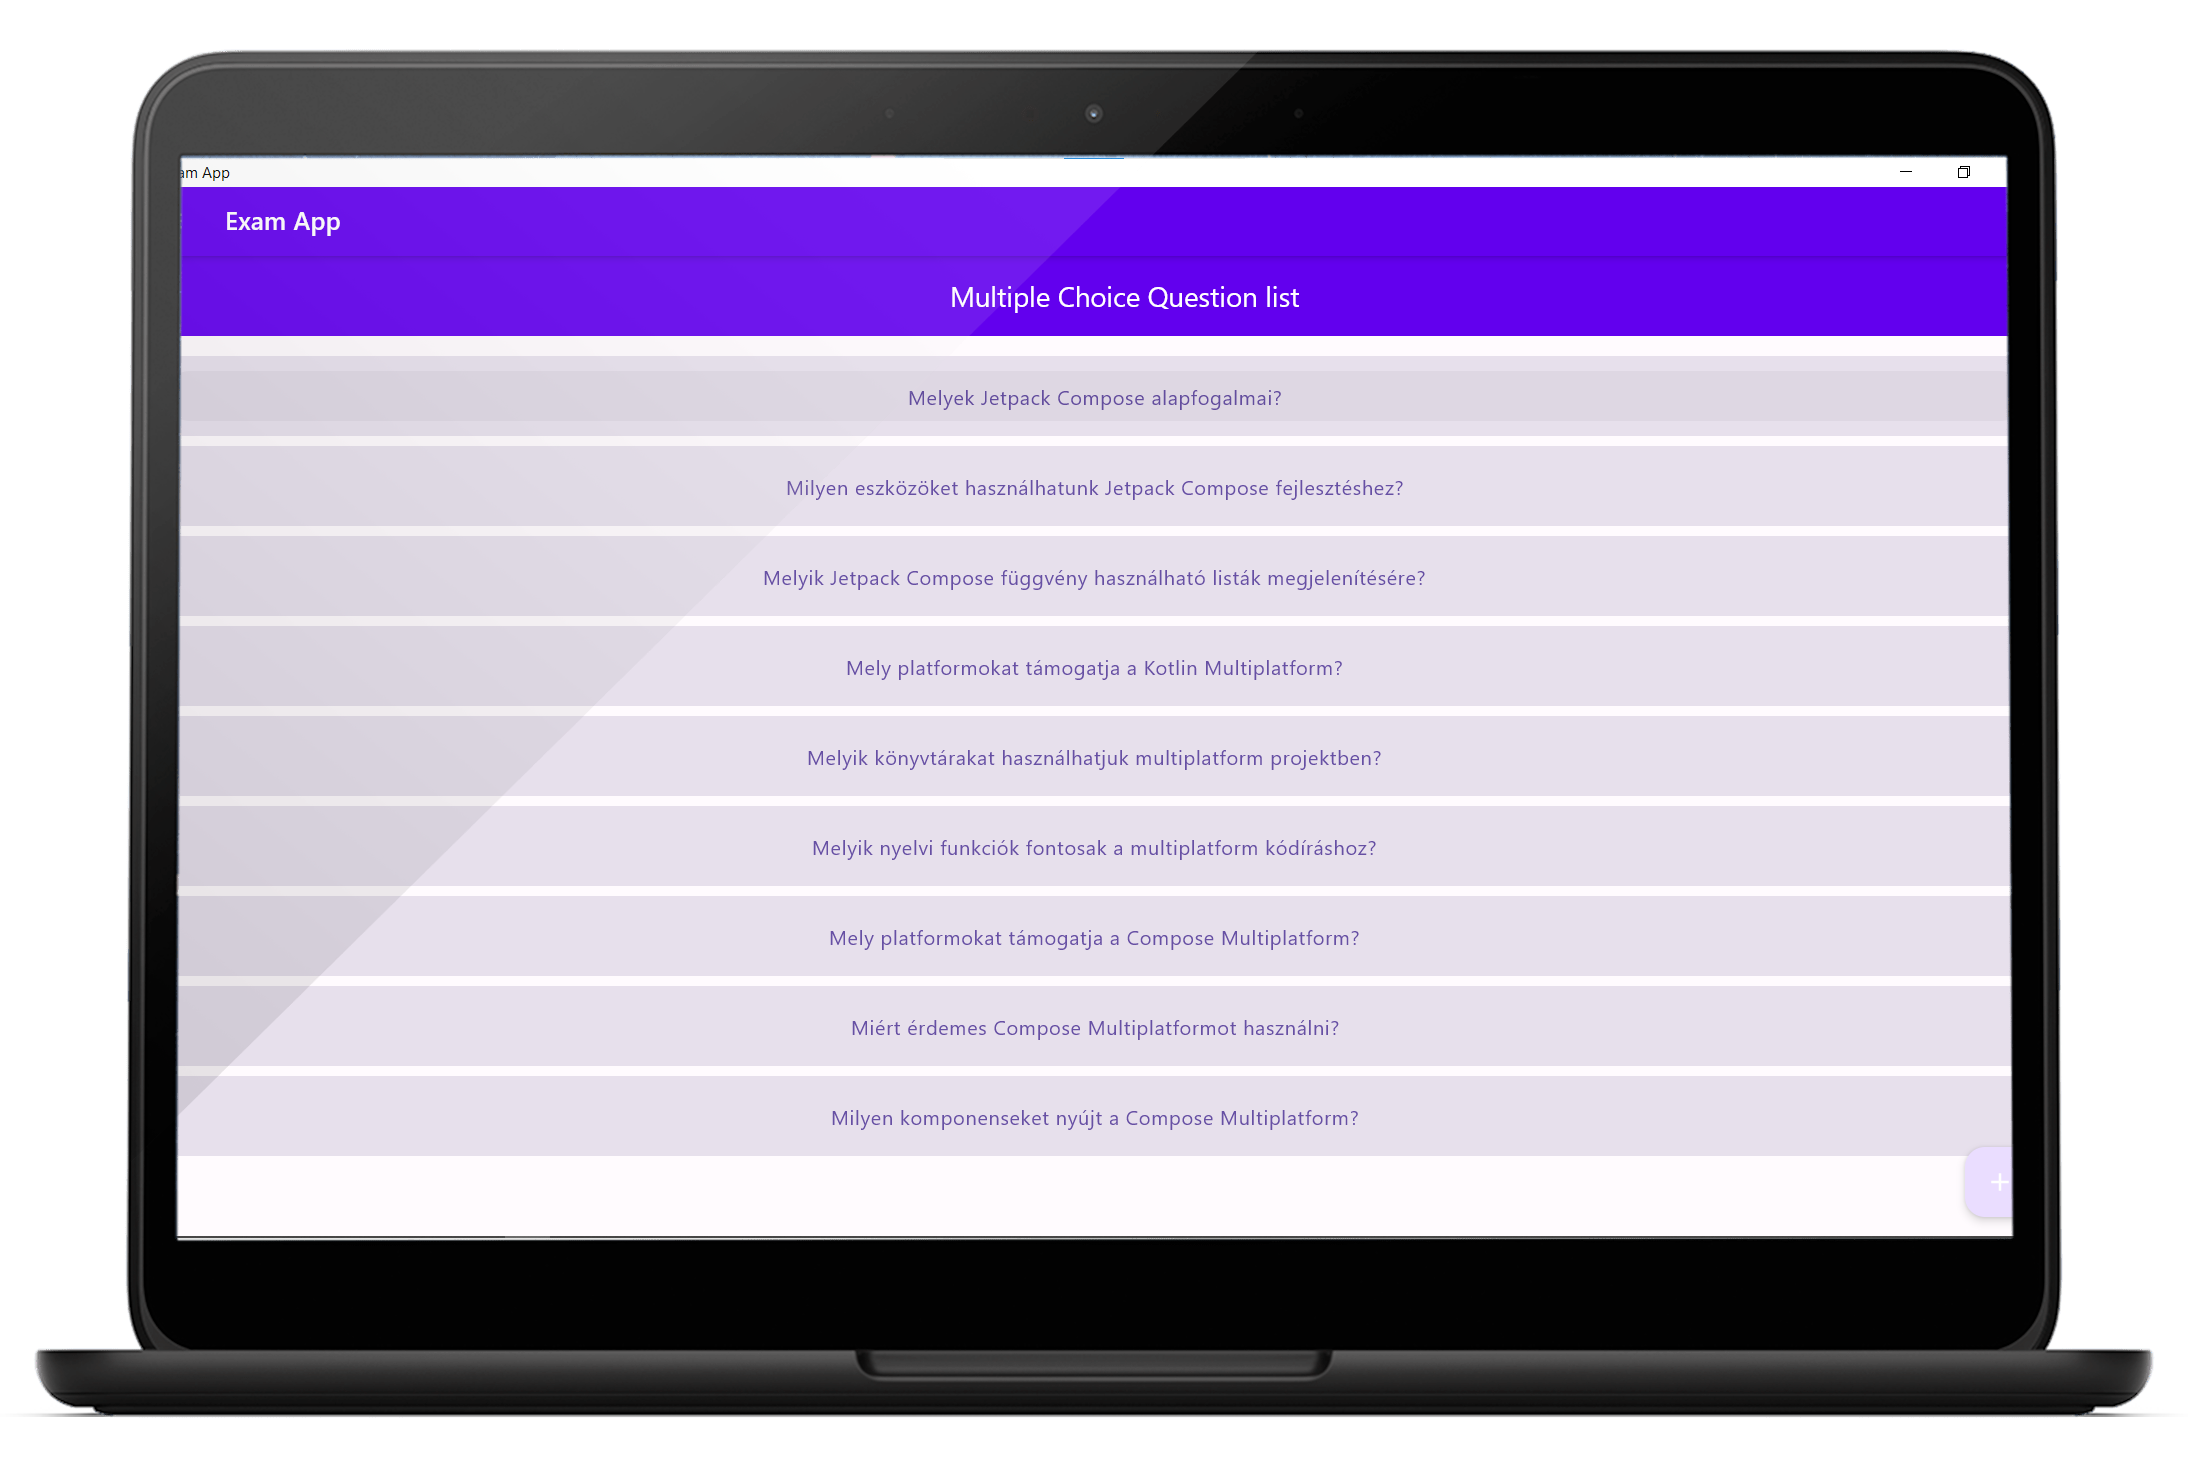
\includegraphics[width=0.6\textwidth, keepaspectratio]{figures/ListView_Desktop_framed.png}
    \end{tabular}
    \caption{A fő képernyő Android és asztali alkalmazáson}
    \label{fig:ListScreen}
\end{figure}


\subsubsection{Részletes nézet}

A részletes oldalak általában csak az összes adatot felsorolják és mutatják meg a felhasználónak.
Ezen kívül tartalmaznak egy törlés opciót ami egy megerősítő ablakot dob fel, mivel a törlés az végleges.
Továbbá innen mehetünk át a szerkesztő oldalra is.

A \refstruc{fig:DetailsScreen} egy érdekesebb megoldást mutat be.
Az oldal tetején a szokásos navigációs sávon kívül elhelyezkedik egy a kérdések közötti keresést segítő rész.
Szűrhetünk kérdéstíusokra, ezt a csúszka segítségével tehetjük meg, ez egyúttal át is színezi azt a könnyebb megkülönböztethetőség kedvéért.
Ezen kívül szűrhetünk témákra is.
Az utolsó dropdwon menü segítségével választhatunk ki egy kérdést amit a gombbal hozzá adhatunk a listához.

A lista része szintén LazyColumn alapú, itt a kérdések típusa alapjén vannak színezve az elemek.
A kérdésekre kattintva lenyílnak és megnézhetjük a legfontosabb adataikat, és innen is lehet törölni a kérdéseket a listából. Ezzel csak a számonkérésből törlődnek, nem a teljes adatbázsiból.
Hosszan lenyomva az elemet elhúzhatjuk felfelé és lefelé ezzel szabadon átrendzhetjük az kérdések sorrendjét.

\begin{lstlisting}[caption={Kinyitható kérdés megvalósítása.}, label={lst:DetailsScreen}, language=Kotlin]
@Composable
fun ExpandableQuestionItem(...){
    var expandedState by remember { mutableStateOf(false) }
    val rotationState by animateFloatAsState(
        targetValue = if (expandedState) 180f else 0f, label = ""
    )
    val coroutineScope = rememberCoroutineScope()
    Card(
        modifier = Modifier.fillMaxWidth()
            .animateContentSize(
                animationSpec = tween(
                    durationMillis = 300,
                    easing = LinearOutSlowInEasing)),
        onClick = { expandedState = !expandedState}
    ) {
        Row(modifier = Modifier.background(if(question.typeOrdinal == Type.trueFalseQuestion.ordinal) PaleDogwood else Green)) {
            Column(...) {
                when (question.typeOrdinal) {
                    Type.trueFalseQuestion.ordinal -> {
                        val trueFalseQuestion = question as TrueFalseQuestionDto
                        if (expandedState) {
                            TrueFalseQuestionDetails(
                                trueFalseQuestion = trueFalseQuestion.toTrueFalseQuestionDetails(...),
                                modifier = Modifier.fillMaxWidth(),
                                colors = CardDefaults.cardColors(
                                    containerColor = PaleDogwood,
                                    contentColor = Purple40
                                )
                            )
                            RemoveButton(coroutineScope, examViewModel, question)
                        } else {
                            CollapsedQuestion(
                                question = trueFalseQuestion.question,
                                containerColor = PaleDogwood, contentColor = Purple40
                        )}}
                    Type.multipleChoiceQuestion.ordinal -> {...}
                }}
                IconButton(modifier = Modifier.weight(1f).alpha(0.2f).rotate(rotationState),
                    onClick = {expandedState = !expandedState}) {
                    Icon(
                        imageVector = Icons.Default.ArrowDropDown,
                        contentDescription = "Drop-Down Arrow"
                )}
        }}}
\end{lstlisting}

A fenti kódrészletben sok érdekes megoldás látható.
Az elején felveszünk több Statet, de ezek közül a második a legizgalamsabb. Ez a State lesz az egyik fontos eleme az animációnak.
Felhasználjuk benne az első Statet aminek az állapota a kérdésre kattintáskot változik, és ennek az értéktől függően (nyitott vagy csukott) változtatjuk az animácihóz tartozó értéket.
A Card Composable elemenhasználjuk az animációt, ezt az animateContentSize segítségével tehetjük meg.
Vannak más fajta animációk is,mindegyik testreszabható és sajátok is létrehozhatóak. Ez esetben egy tween animációt használunk ami 0.3 másodperc alatt az összecsukott állpotról egy nyitott állapotra áll át.
Attól változik meg az elem és játszódik le az animáció, hogy rákattintunk a kérdésre.
Mivel a Cardon az animateContentSizet használtuk ezért amikor az expandedState megváltozok akkor a CollapsedQuestion helyett a recomposoition után a TrueFalseQuestionDetails kell megjeleníteni ez méretváltozással jár, ezt követi le az animáció ezáltal nem hirtelen ugrik egyet a képrenyő, hanem lekövethető módon változik meg.
A rotationState pedig az ArrowDropDown elem animálásban játszik szerepet, így az ikont el tudjuk forgatni 180 fokkal, ehhez a Modifierhez tartozó rotate(Int) extension functiont tudjuk használni.

\begin{figure}[!ht]
    \centering
    \begin{tabular}{cc}
        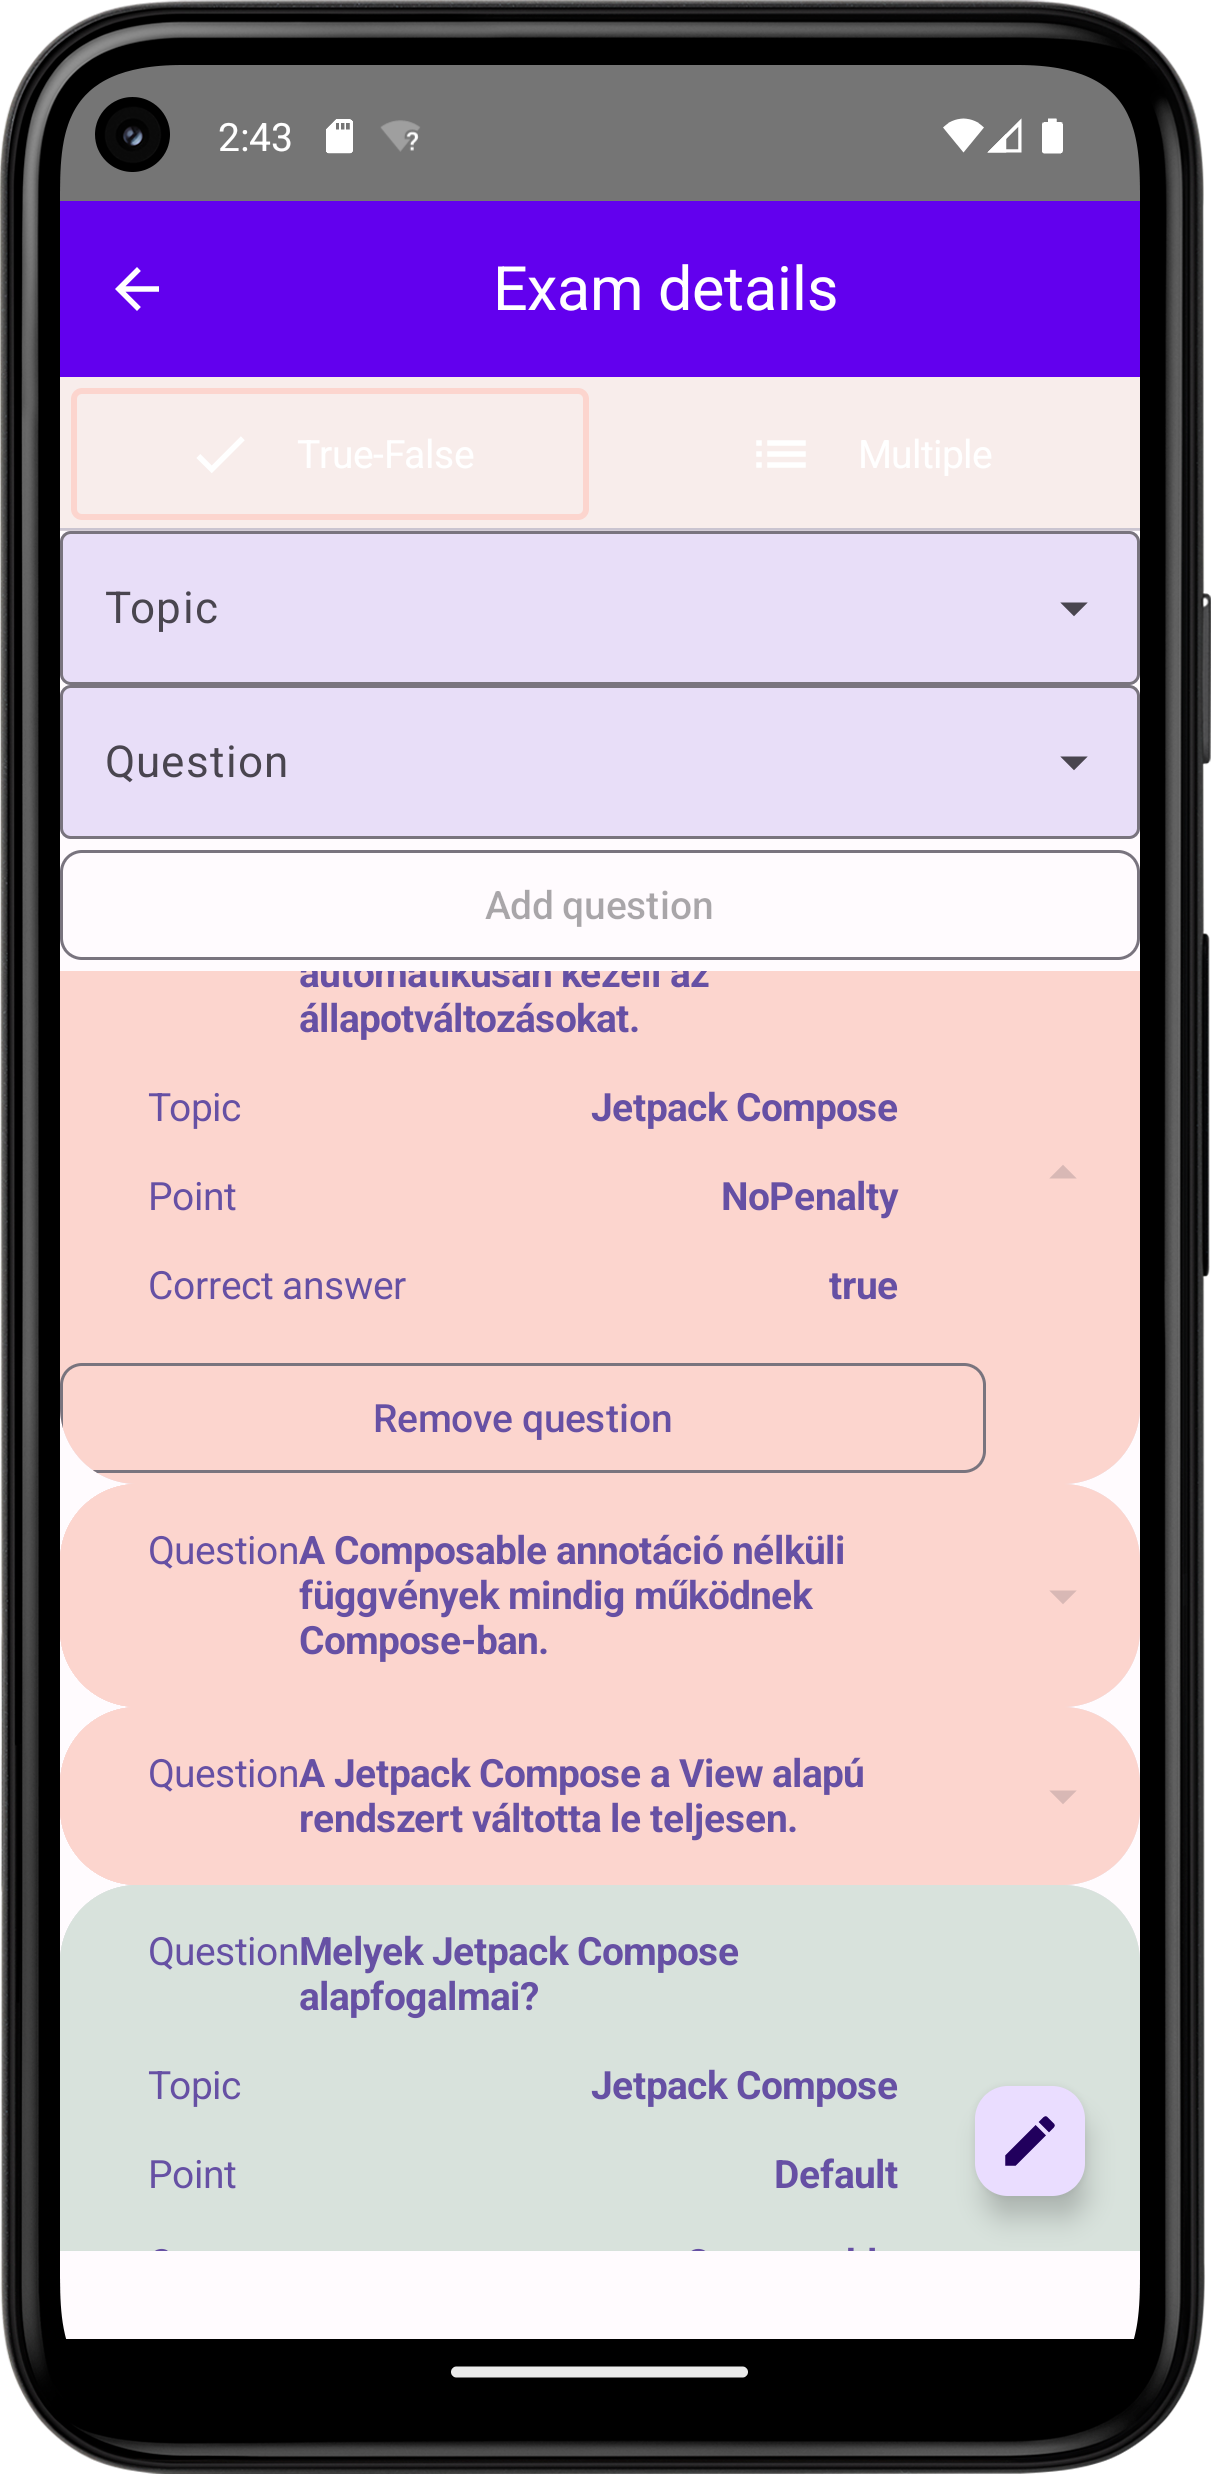
\includegraphics[width=0.3\textwidth, keepaspectratio]{figures/Details_Android.png} & 
        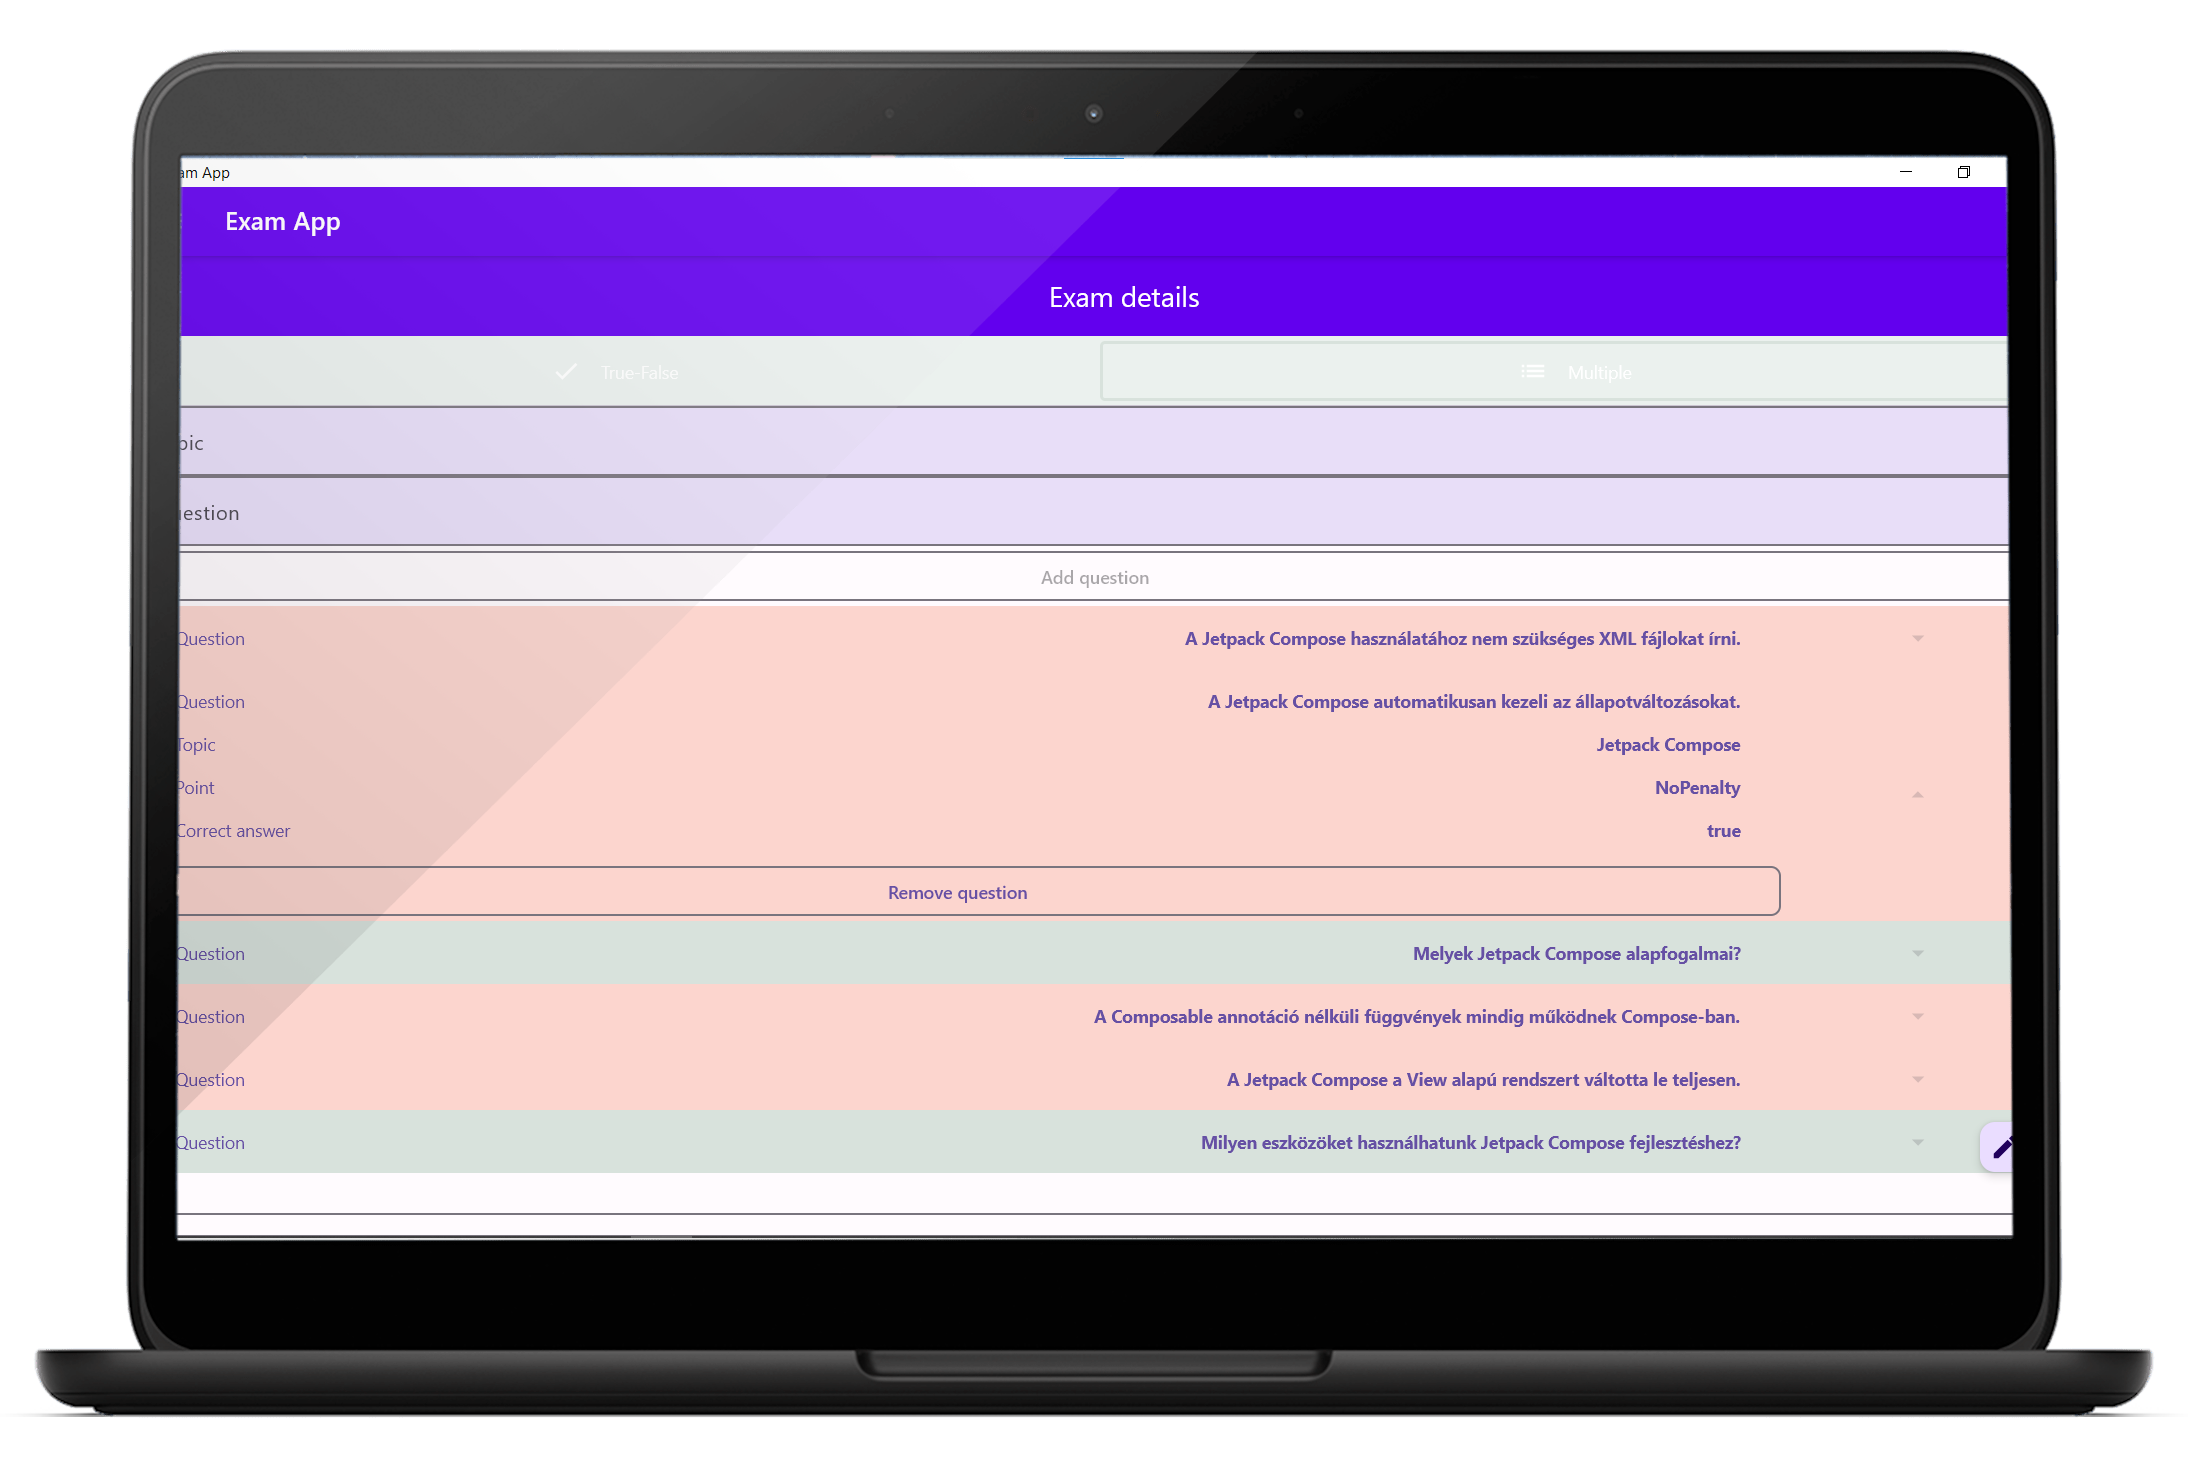
\includegraphics[width=0.6\textwidth, keepaspectratio]{figures/Details_Desktop_framed.png}
    \end{tabular}
    \caption{Egy érdekesebb részletes képernyő, a vizsgák összeállításához tartozik.}
    \label{fig:DetailsScreen}
\end{figure}


\subsubsection{Szerekesztő nézet}

\begin{figure}[!ht]
    \centering
    \begin{tabular}{cc}
        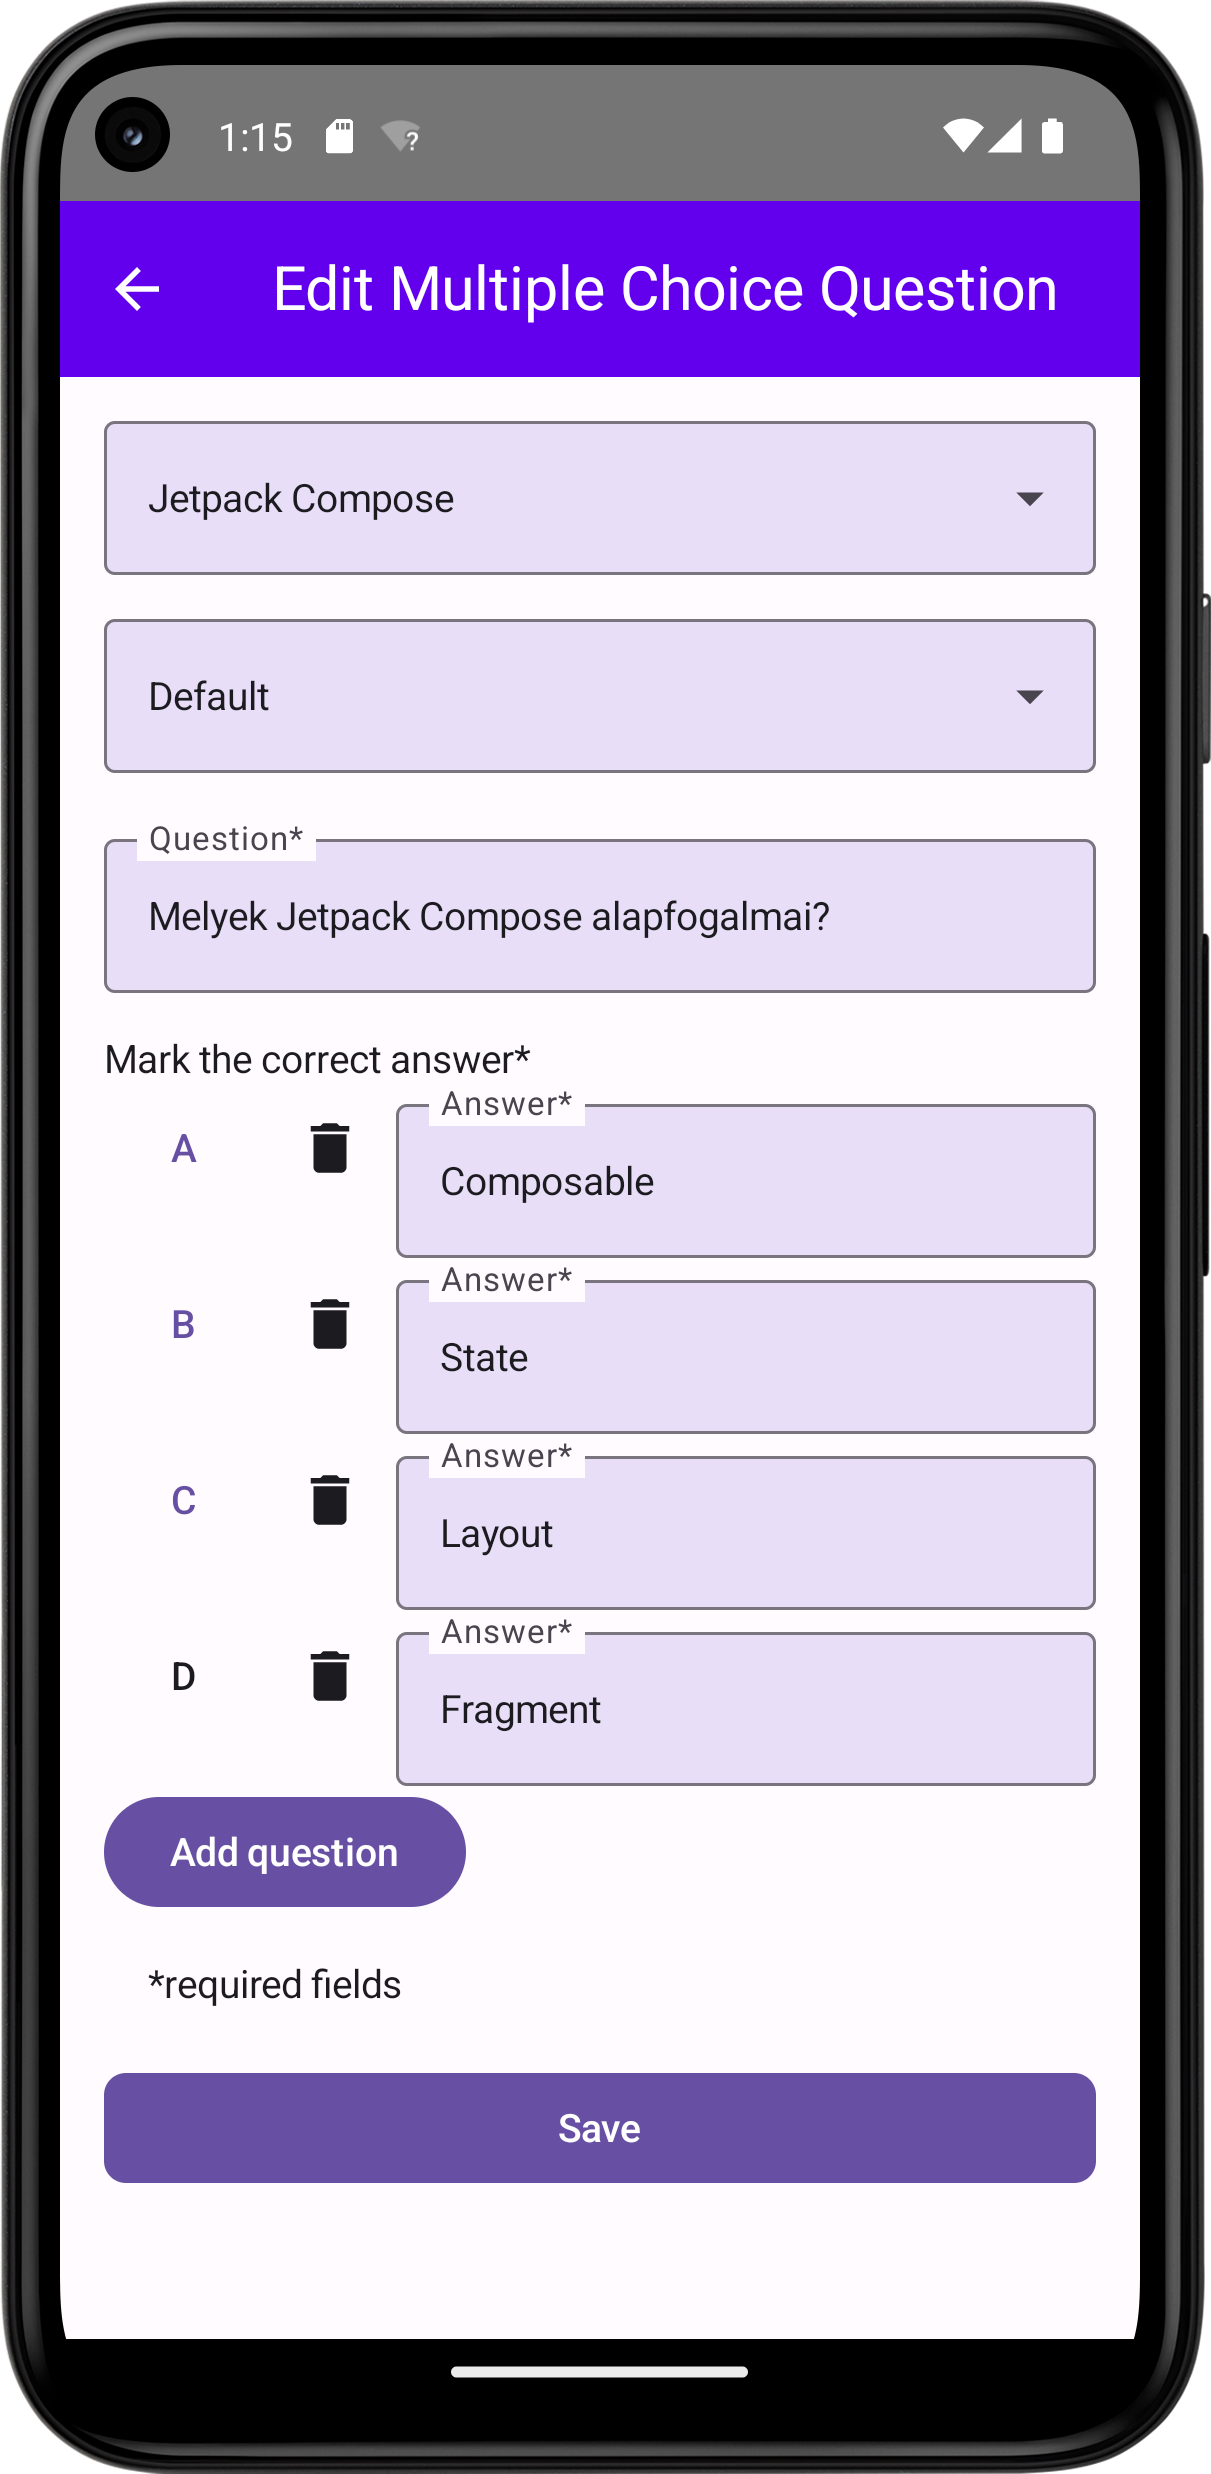
\includegraphics[width=0.3\textwidth, keepaspectratio]{figures/Edit_Android.png} & 
        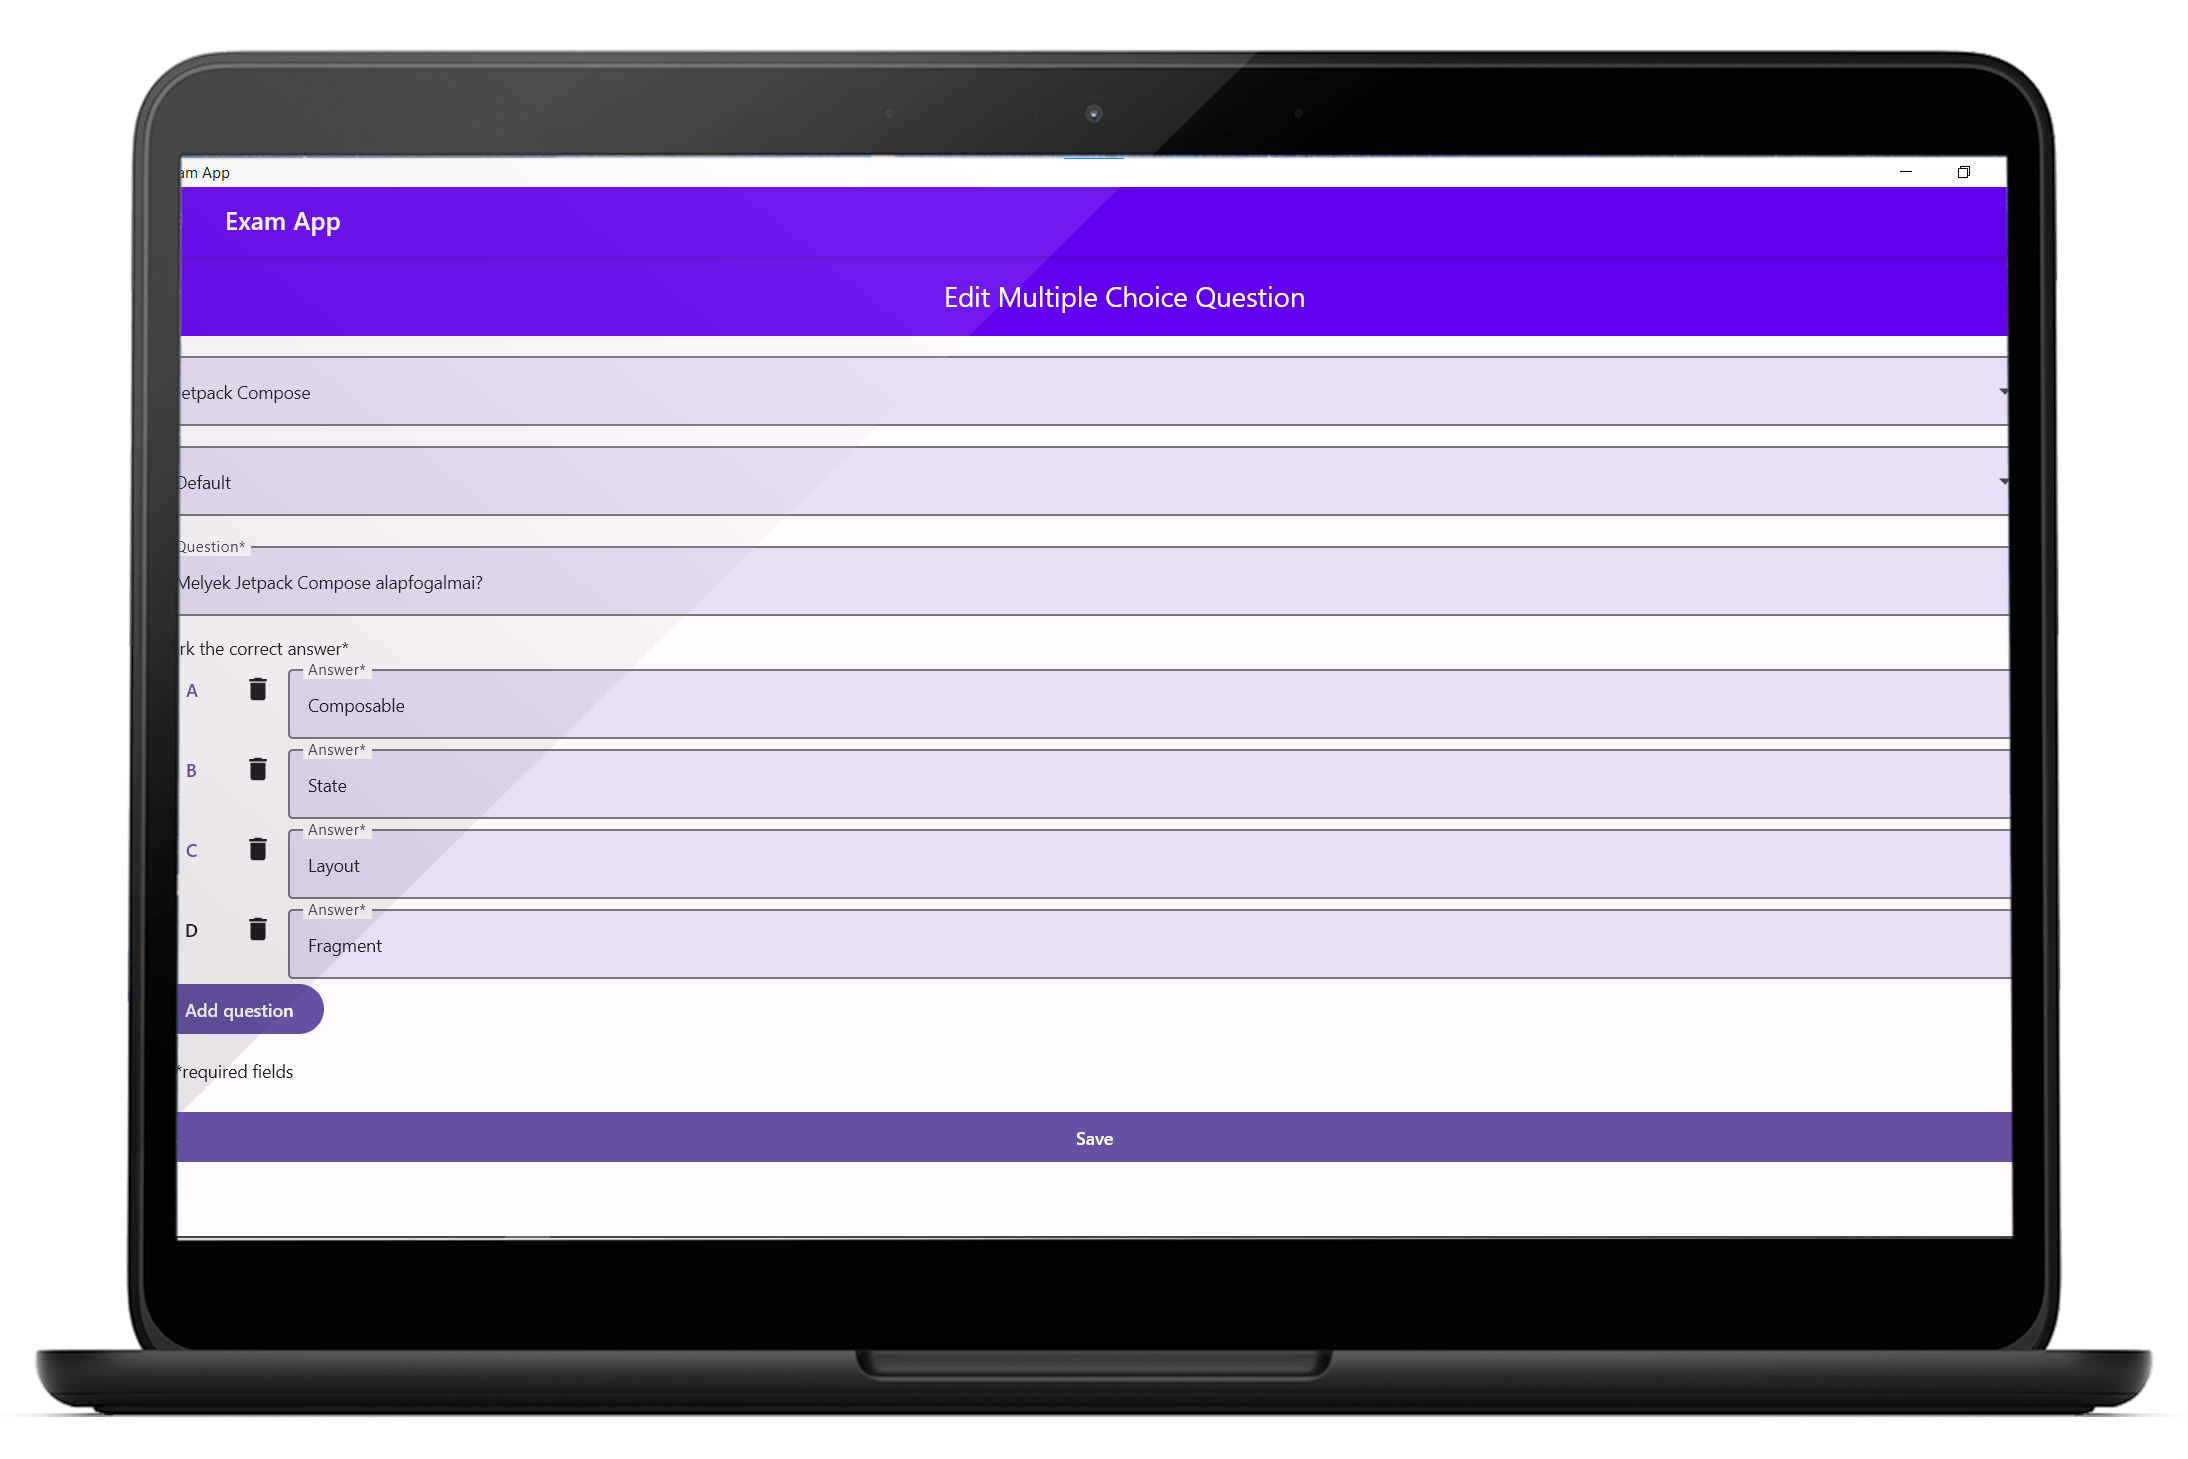
\includegraphics[width=0.6\textwidth, keepaspectratio]{figures/Edit_Desktop_framed.png}
    \end{tabular}
    \caption{Egy érdekesebb szerkesztő képernyő, a feleltválasztós kérdések létrehozásához.}
    \label{fig:EditScreen}
\end{figure}

A szerkesztő nézetben lehet módosítani minden adtot (kivéve a feladatsorhoz tartozó kérdéseket, amit az előző alfejezetben mutattam be).
Itt sok féle elem megtaláható; szöveges bevuteli mezők, dropdwon menü, a pontok esetében pedig numerikus beviteli mezők.

A feleletválasztós kérdéseknél (\refstruc{fig:EditScreen}) van egy sepciális elem, ami a a kérdések megadásához készült.
Tartalmaz egy TextButtont, ami a válasz sorszáma, egy ImageButton a válsz törléséhez és egy szöveges beviteli mező a válasz megadásához.
Tetszőlges opció megadható, itt viszont egy egyszerű Column mellet döntöttem és egy for ciklus segítségével rajzolom ki az elemket.


\begin{lstlisting}[caption={Szerkesztő nézet kódja.}, label={lst:EditScreen}, language=Kotlin]
@Composable
fun ExamInputForm(
    enabled: Boolean = true,
    entryViewModel: ExamEntryViewModel = viewModel { ExamEntryViewModel() },    
    topicListViewModel: TopicListViewModel = viewModel { TopicListViewModel() },
    ) {
    val coroutineScope = rememberCoroutineScope()
    Column(...) {
        OutlinedTextField(
            value = examDetails.name,
            onValueChange = { onValueChange(examDetails.copy(name = it)) },
            enabled = enabled,
            ...
        )
        DropDownList(
            name = stringResource(Res.string.exam),
            items = topicListViewModel.topicListUiState.topicList.map{it.topic}.filterNot{ it == examDetails.topicName },
            onChoose = {topic ->
                coroutineScope.launch{
                    onValueChange(examDetails.copy(topicId = entryViewModel.getTopicIdByTopic(topic)))
                }
            },
            default = examDetails.topicName,
            modifier = Modifier.fillMaxWidth(),
        )
        if (enabled) {
            Text(
                text = stringResource(Res.string.required_fields),
                modifier = Modifier.padding(start = 16.dp)
            )
        }
    }
}
\end{lstlisting}

A fenti kódrészletben megfigyelhetjük a ViewModelek átadását a Composable függvéynek.
Eseténként többre is szükseg lehet, itt például az examEntry és a topicList ViewModelekre is szükség van, mivel a dropdwon listában a témakört ki kell választani a feladatsorhoz.
A dropdwon menü kódjában kihasználtam a kotlin funkciionális programozást segítő kódját, ezzel kigyűjtöttem a témakörök listájából azokat amik nem egyeznek meg a jelenleg kiválasztottal.
A hosszabb ideig tartó műveleteket egy coroutineScopeban valósítáttam meg egy másik lambda függvényben, így a UI nem blokkolódik le közben.
A mentés gomb le van tiltva, ha hiányzik egy kötelező mező vagy ha ez egyedi mezőkben ütközés van a felhasználó kap egy értesítést és a gomb is letiltódik amíg nem változtat az értéken.

\pagebreak

\subsubsection{Új elem létrehozása}

Ez a nézet lényegében megegyezik a szerkesztő nézettel.
Egy jó szoftver arról ismerszik meg, hogy a lehető legtöbb helyen újra felhasználja a már meglévő kódot anélkül, hogy annak a kódját lényegesen meg kelljen változtatnia.
Ebben az eseetben már terevezés során megszületett a dönés. Egész pontosan van egy Body része az új elem felvételének ami vár paraméternek egy UiStateet, amiben az adott elem adatai kerülnek.
Az alapérteki úgy vannak megválasztva, hogy az üres hatást keltsen, de ha már léteznek akkor a szerkesztő nézetet kapjuk, az új létrehozésa helyett.
Ehhez szükség van külön ViewModelre és kevés Composable függvény megírására is, de ez jelentősen kevesebb, mint az egész kód újraírása. Ezzel a kód karbantarhatósága is növekszik.  

\begin{figure}[!ht]
    \centering
    \begin{tabular}{cc}
        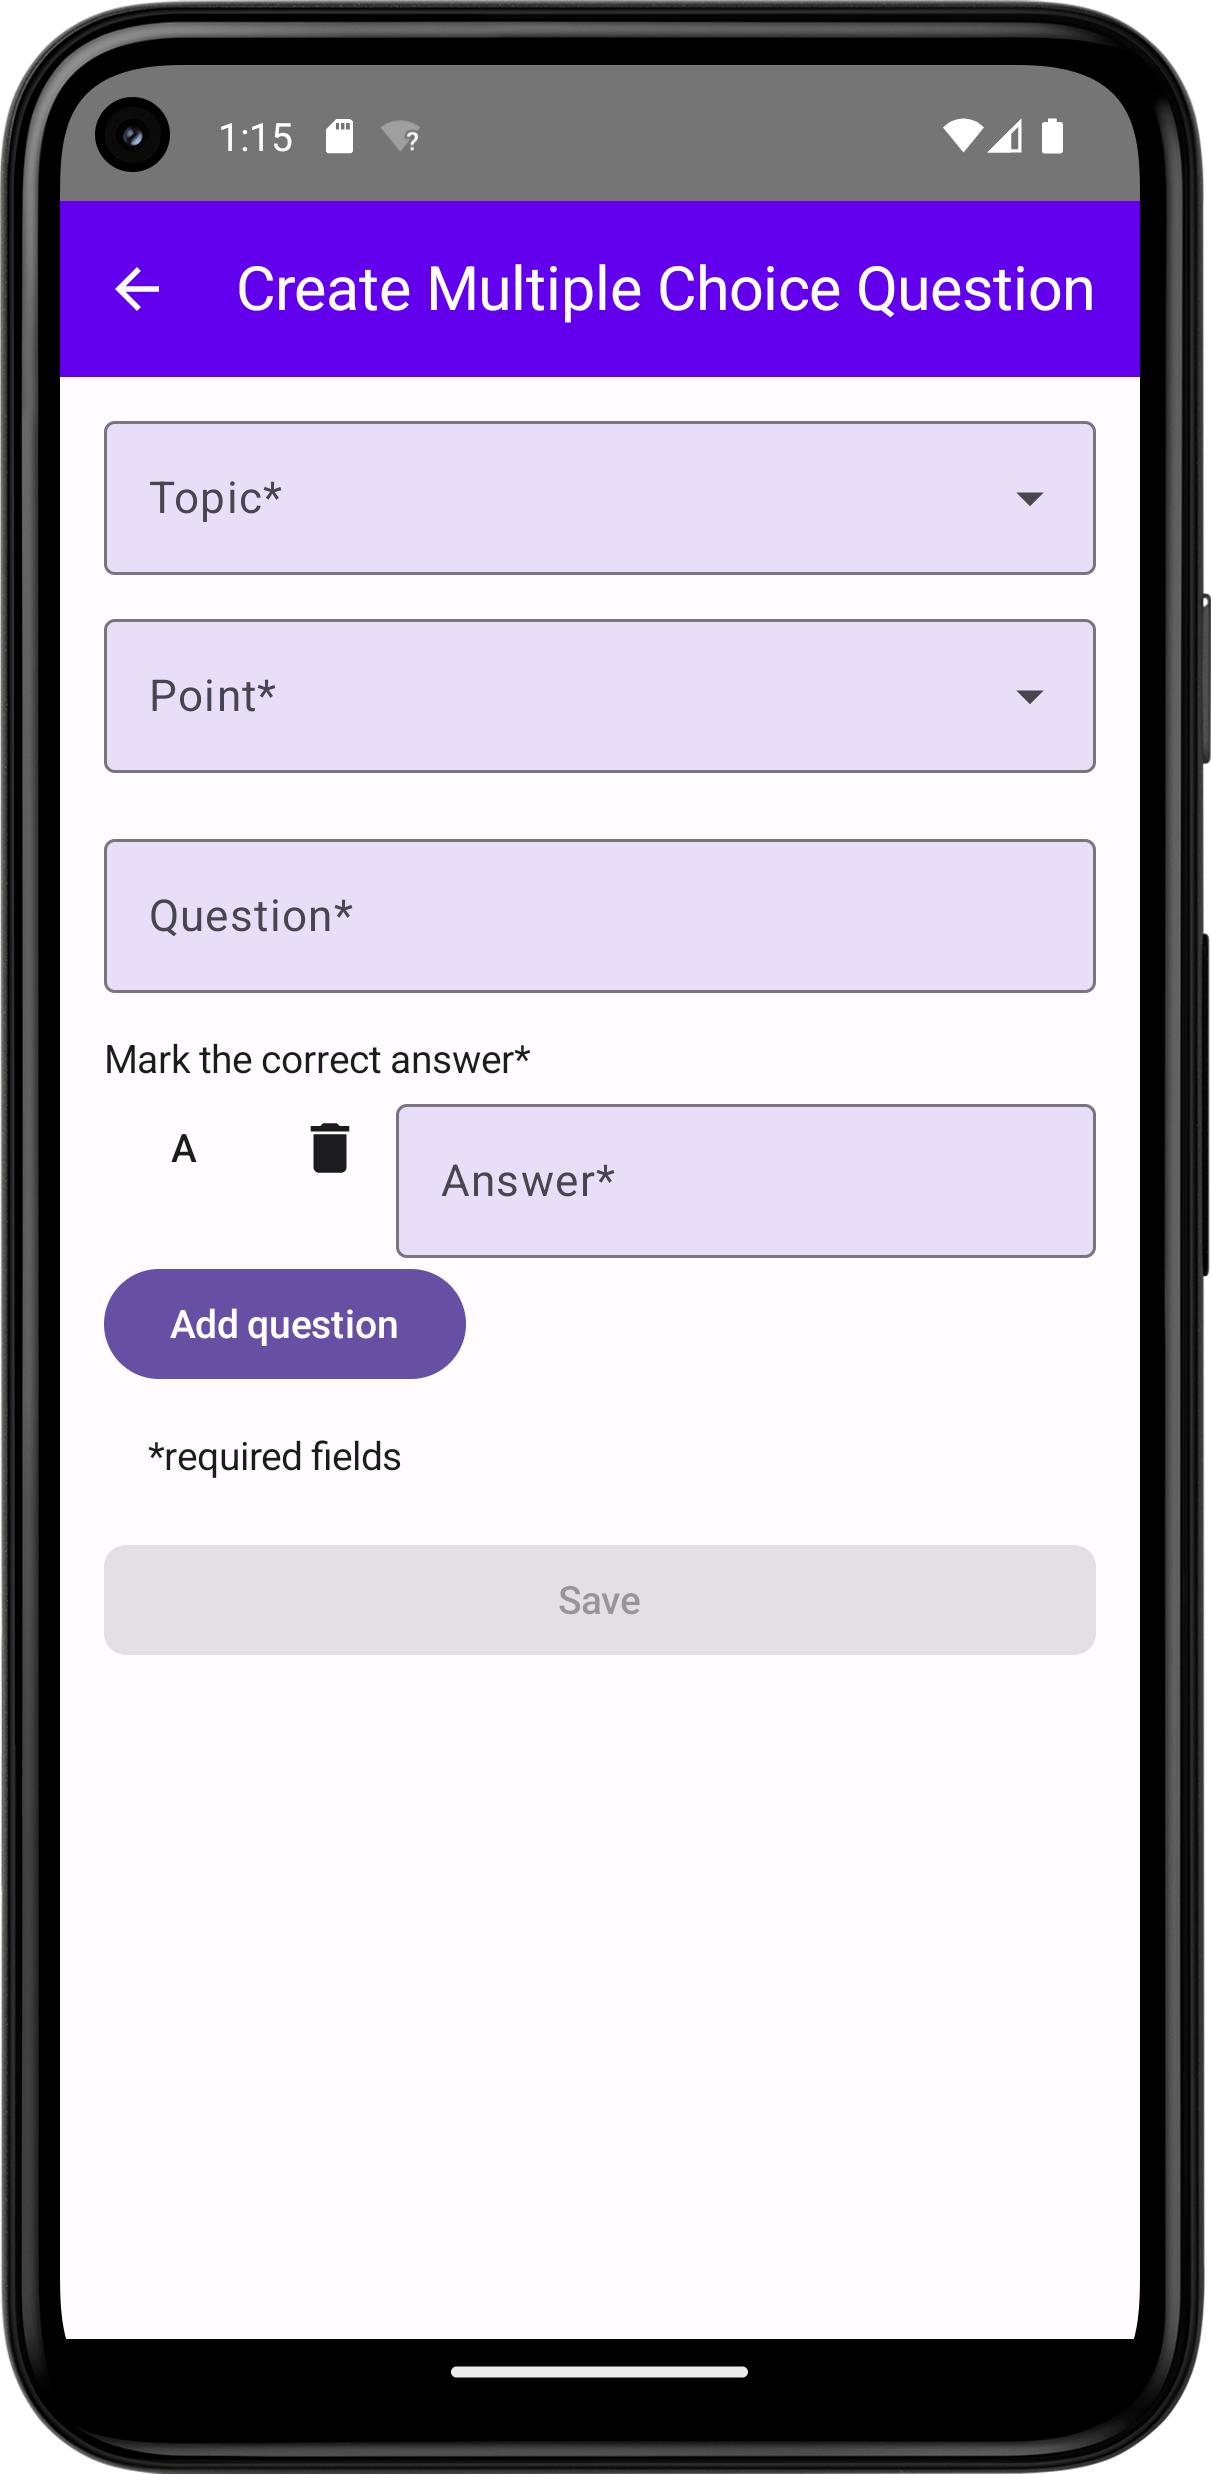
\includegraphics[width=0.3\textwidth, keepaspectratio]{figures/New_Android.png} & 
        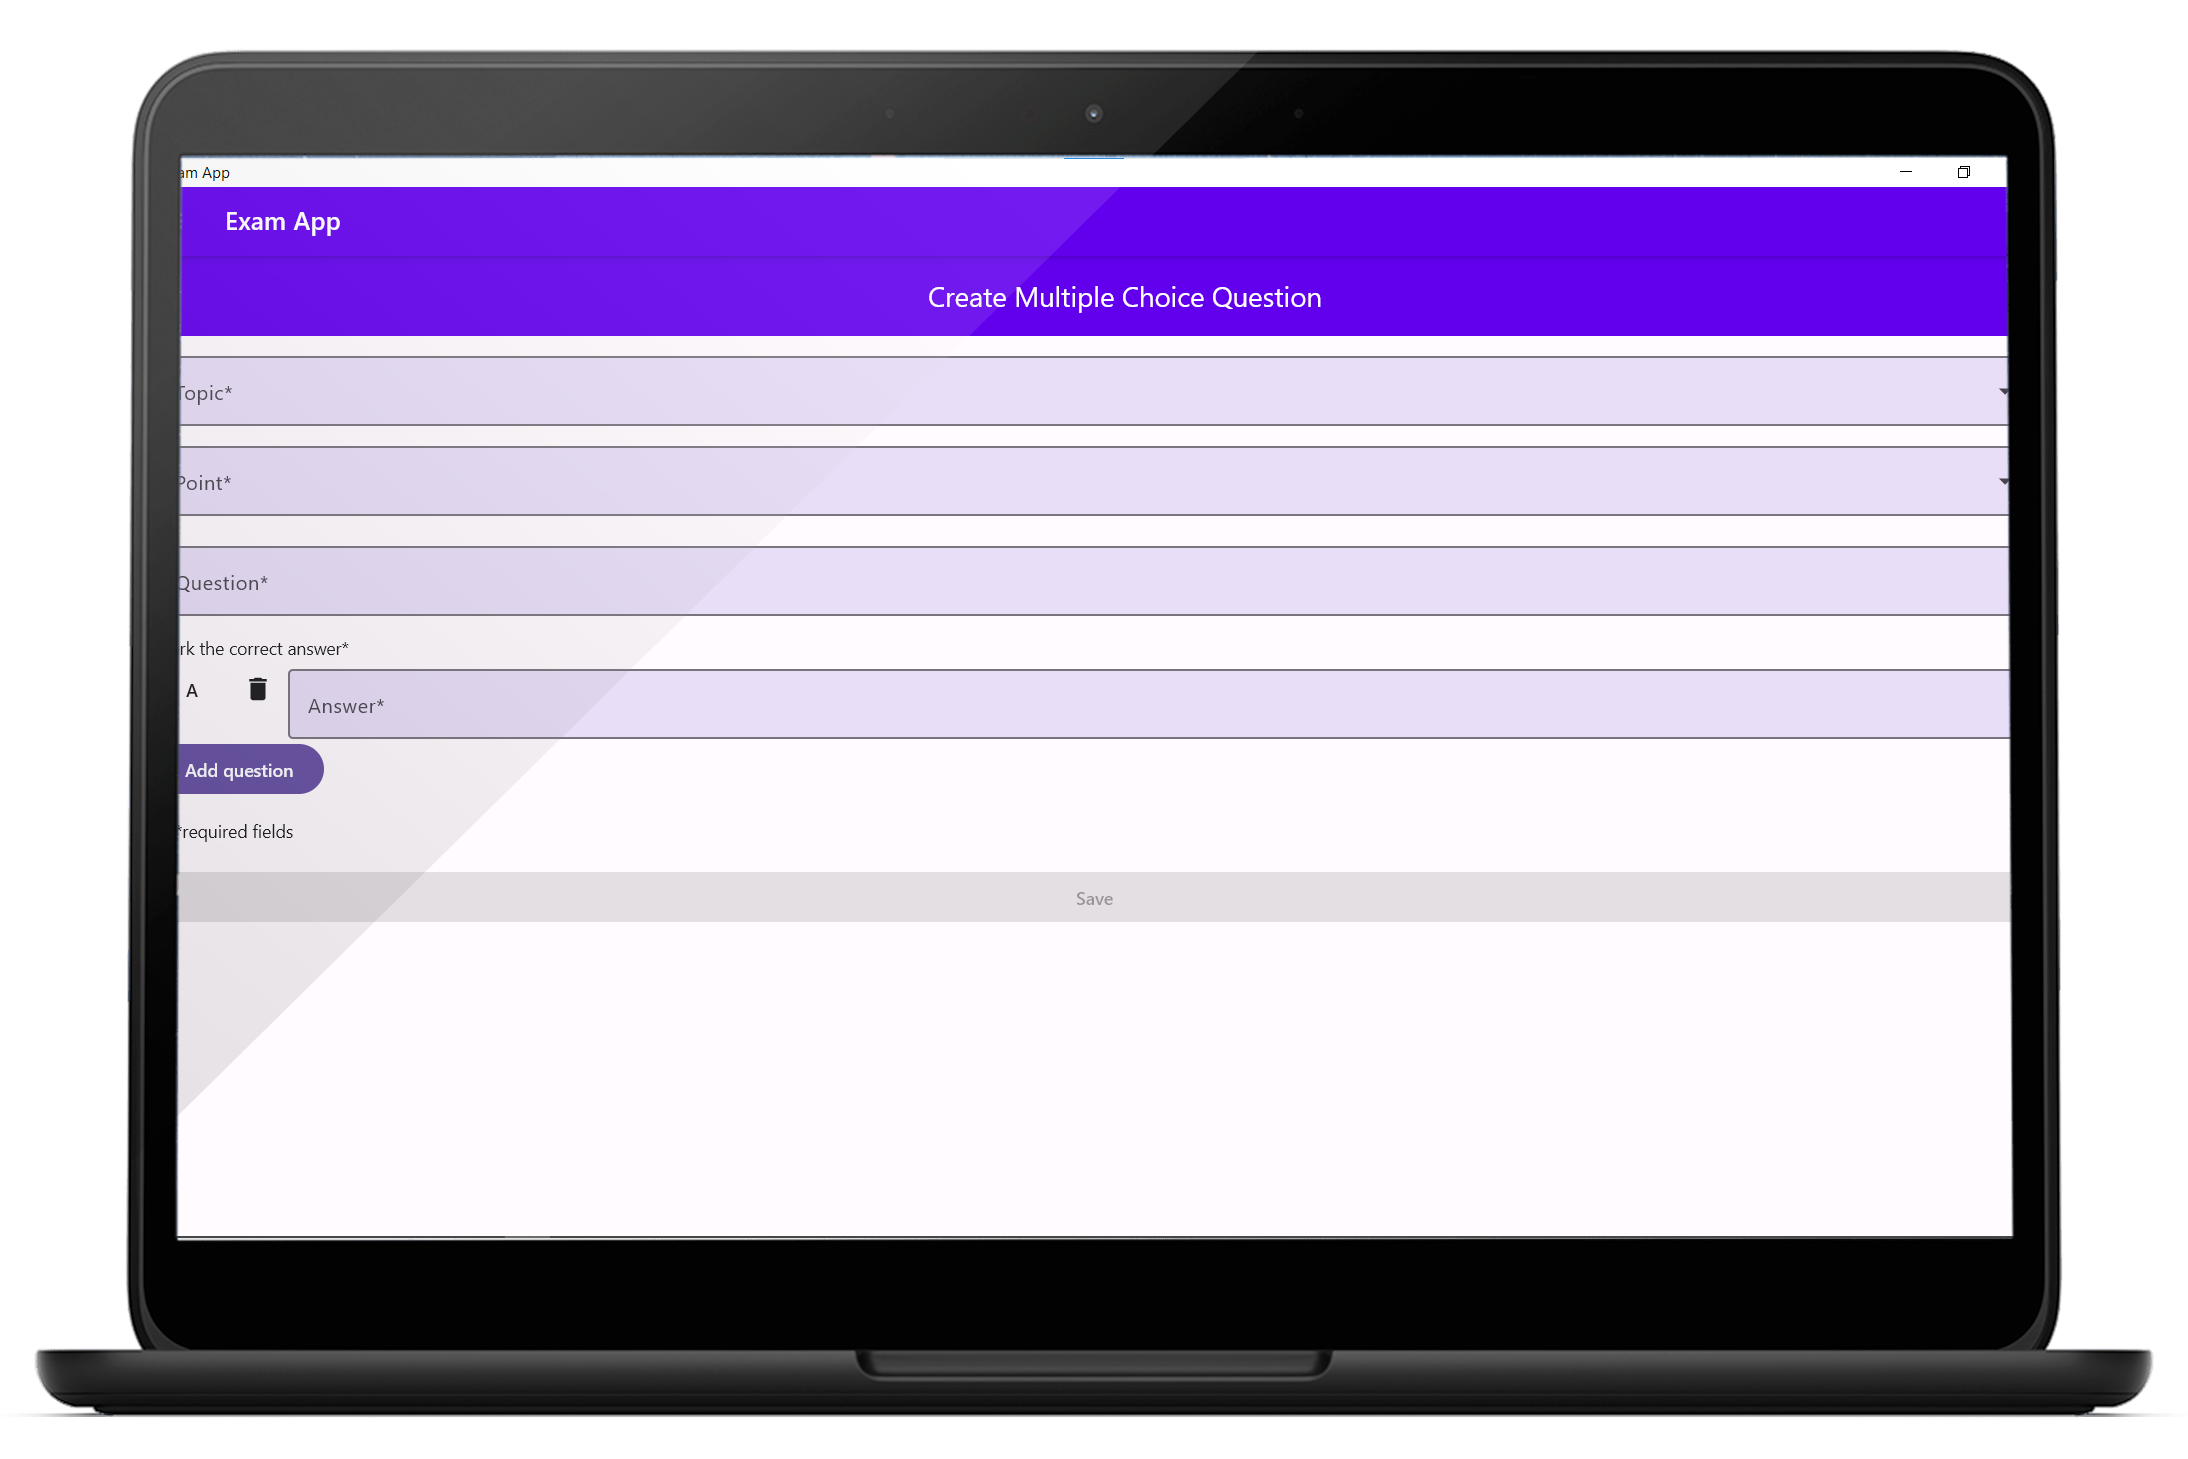
\includegraphics[width=0.6\textwidth, keepaspectratio]{figures/New_Desktop_framed.png}
    \end{tabular}
    \caption{Új feleletválasztós kérdés létrehozása.}
    \label{fig:NewScreen}
\end{figure}


\subsubsection{Ellenőrző képernyő}

Az ellenőrző képetnyőn a kérdések vannak felsorolva, a szokásos színkódolással.
Olvasható a teljes szöveg és a válaszok is a feleltválasztós kérdésknél. 
A válasz formátuma látható kitöltés előtt, így a felhasználó tudja, hogy milyen formátumban van elvárva a válasz.
A fenti Scan Exam gomb Android eszközön megnyit egy kamera nézetet ami segítségével pár gyors mozdulattal be tudjuk olvasni a válaszokat így nem kell kézzel begépelni azt.
Ha valamit nem vagy rosszul detektált a mesterséges intelligencia akkor természtesen az oldalon ezek javíthatóak.
A lap alján található egy gomb ami segítségével ki lehet értékelni a válaszkat, ez a backend oldalon történik meg, majd az eredményt visszaküldi és a felhasznló megtekintheti az elért pontszámot és a százalékos értéket.

\begin{figure}[!ht]
    \centering
    \begin{tabular}{cc}
        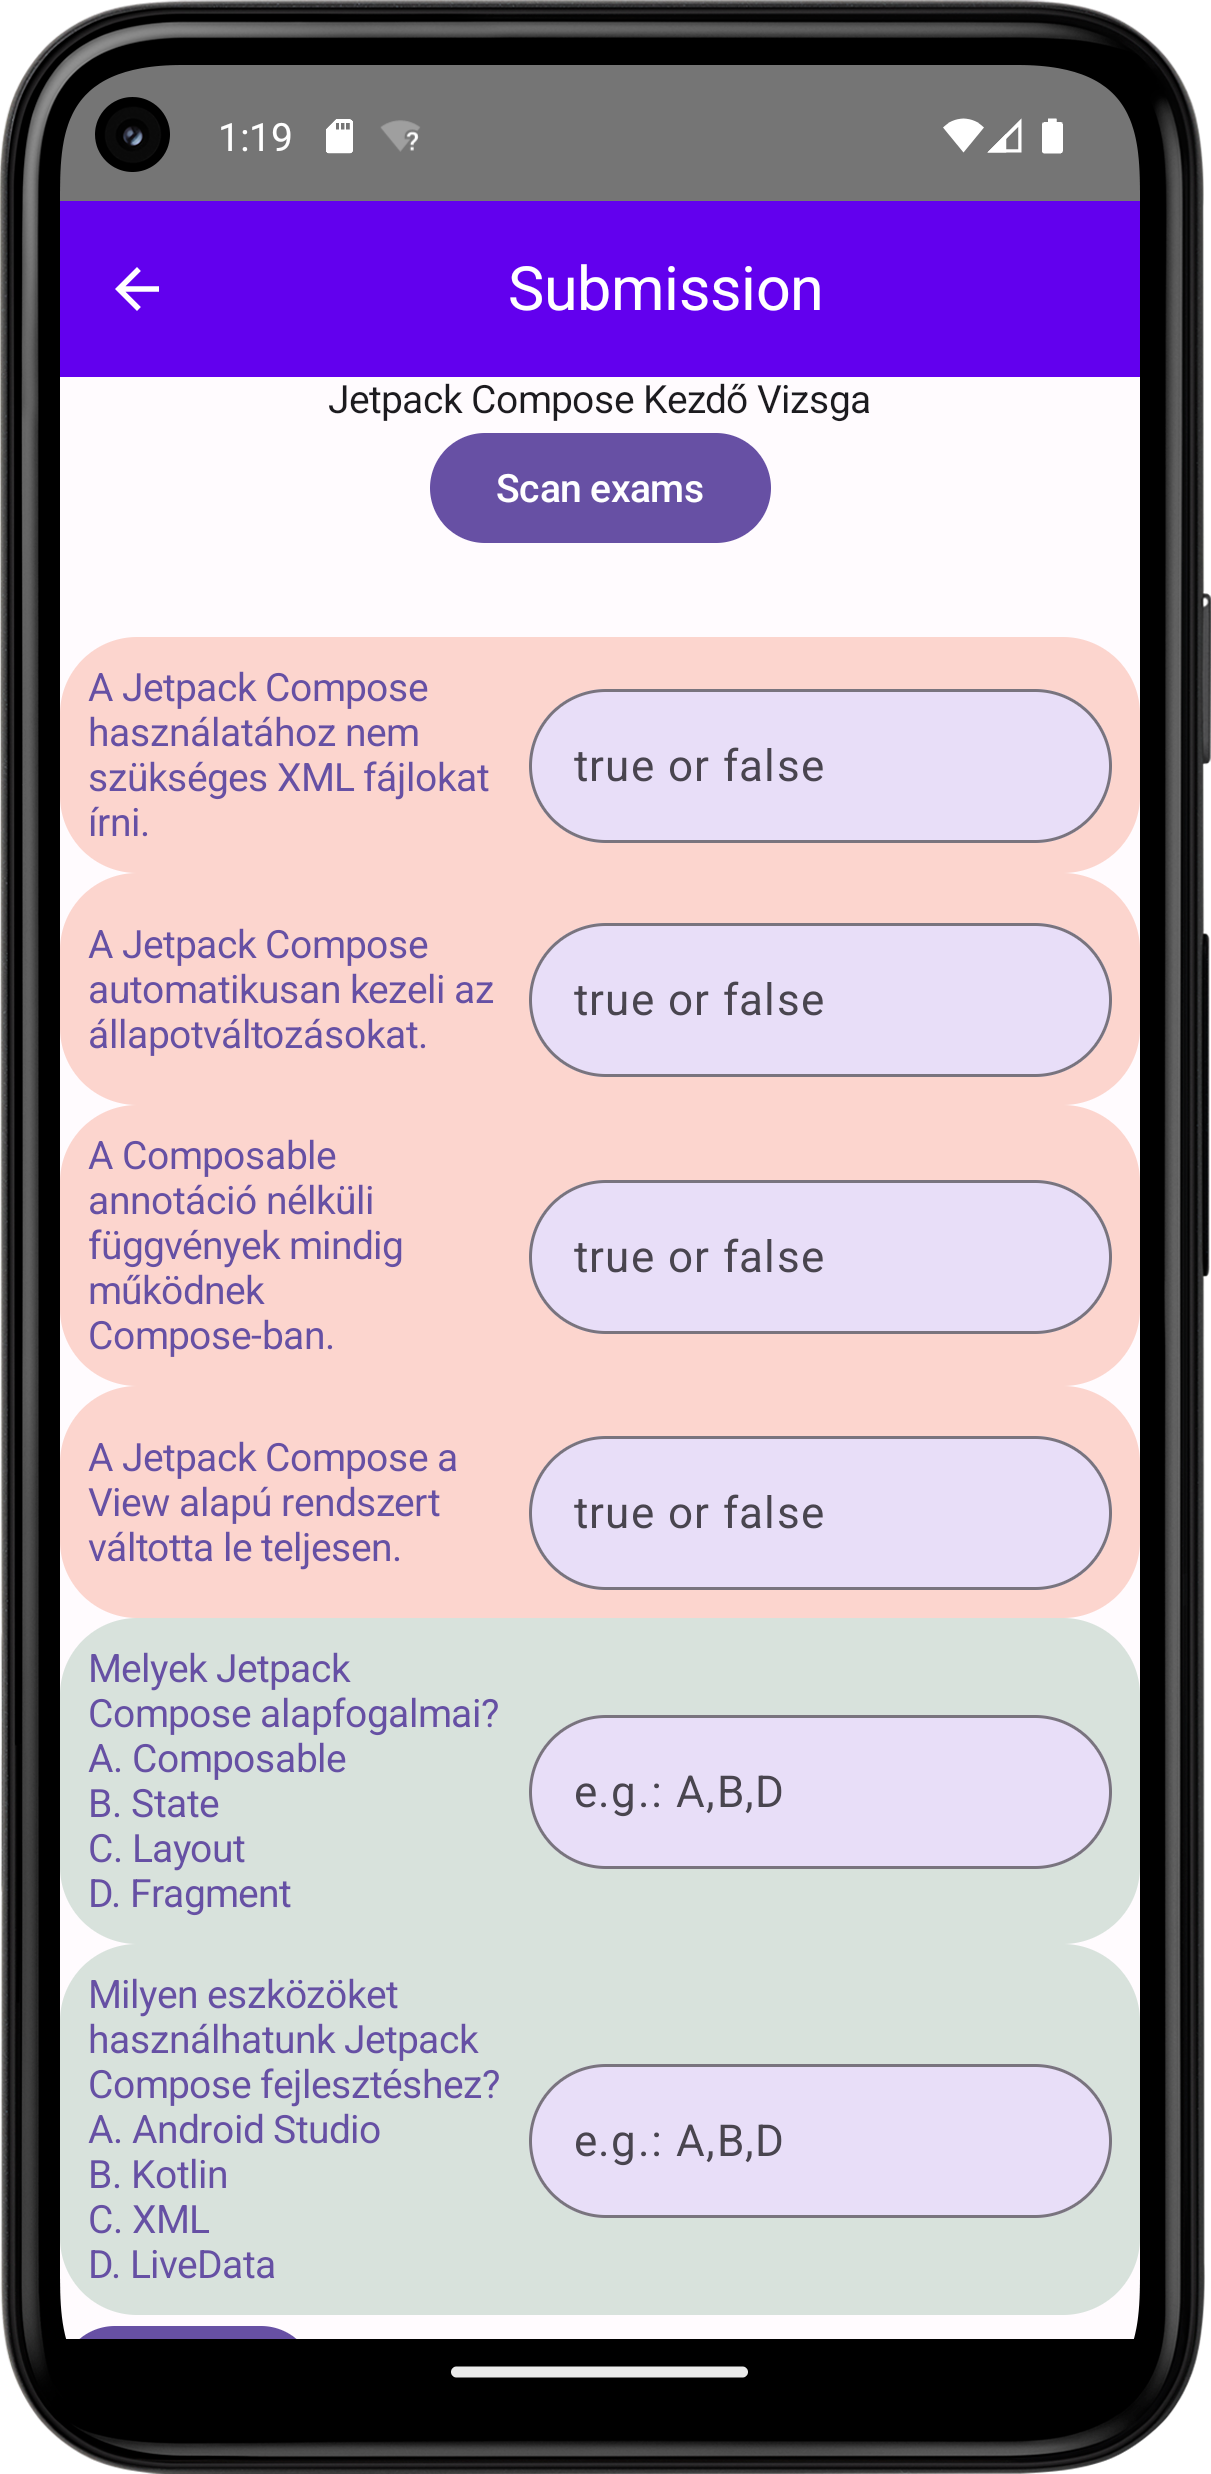
\includegraphics[width=0.3\textwidth, keepaspectratio]{figures/Submission_Android.png} & 
        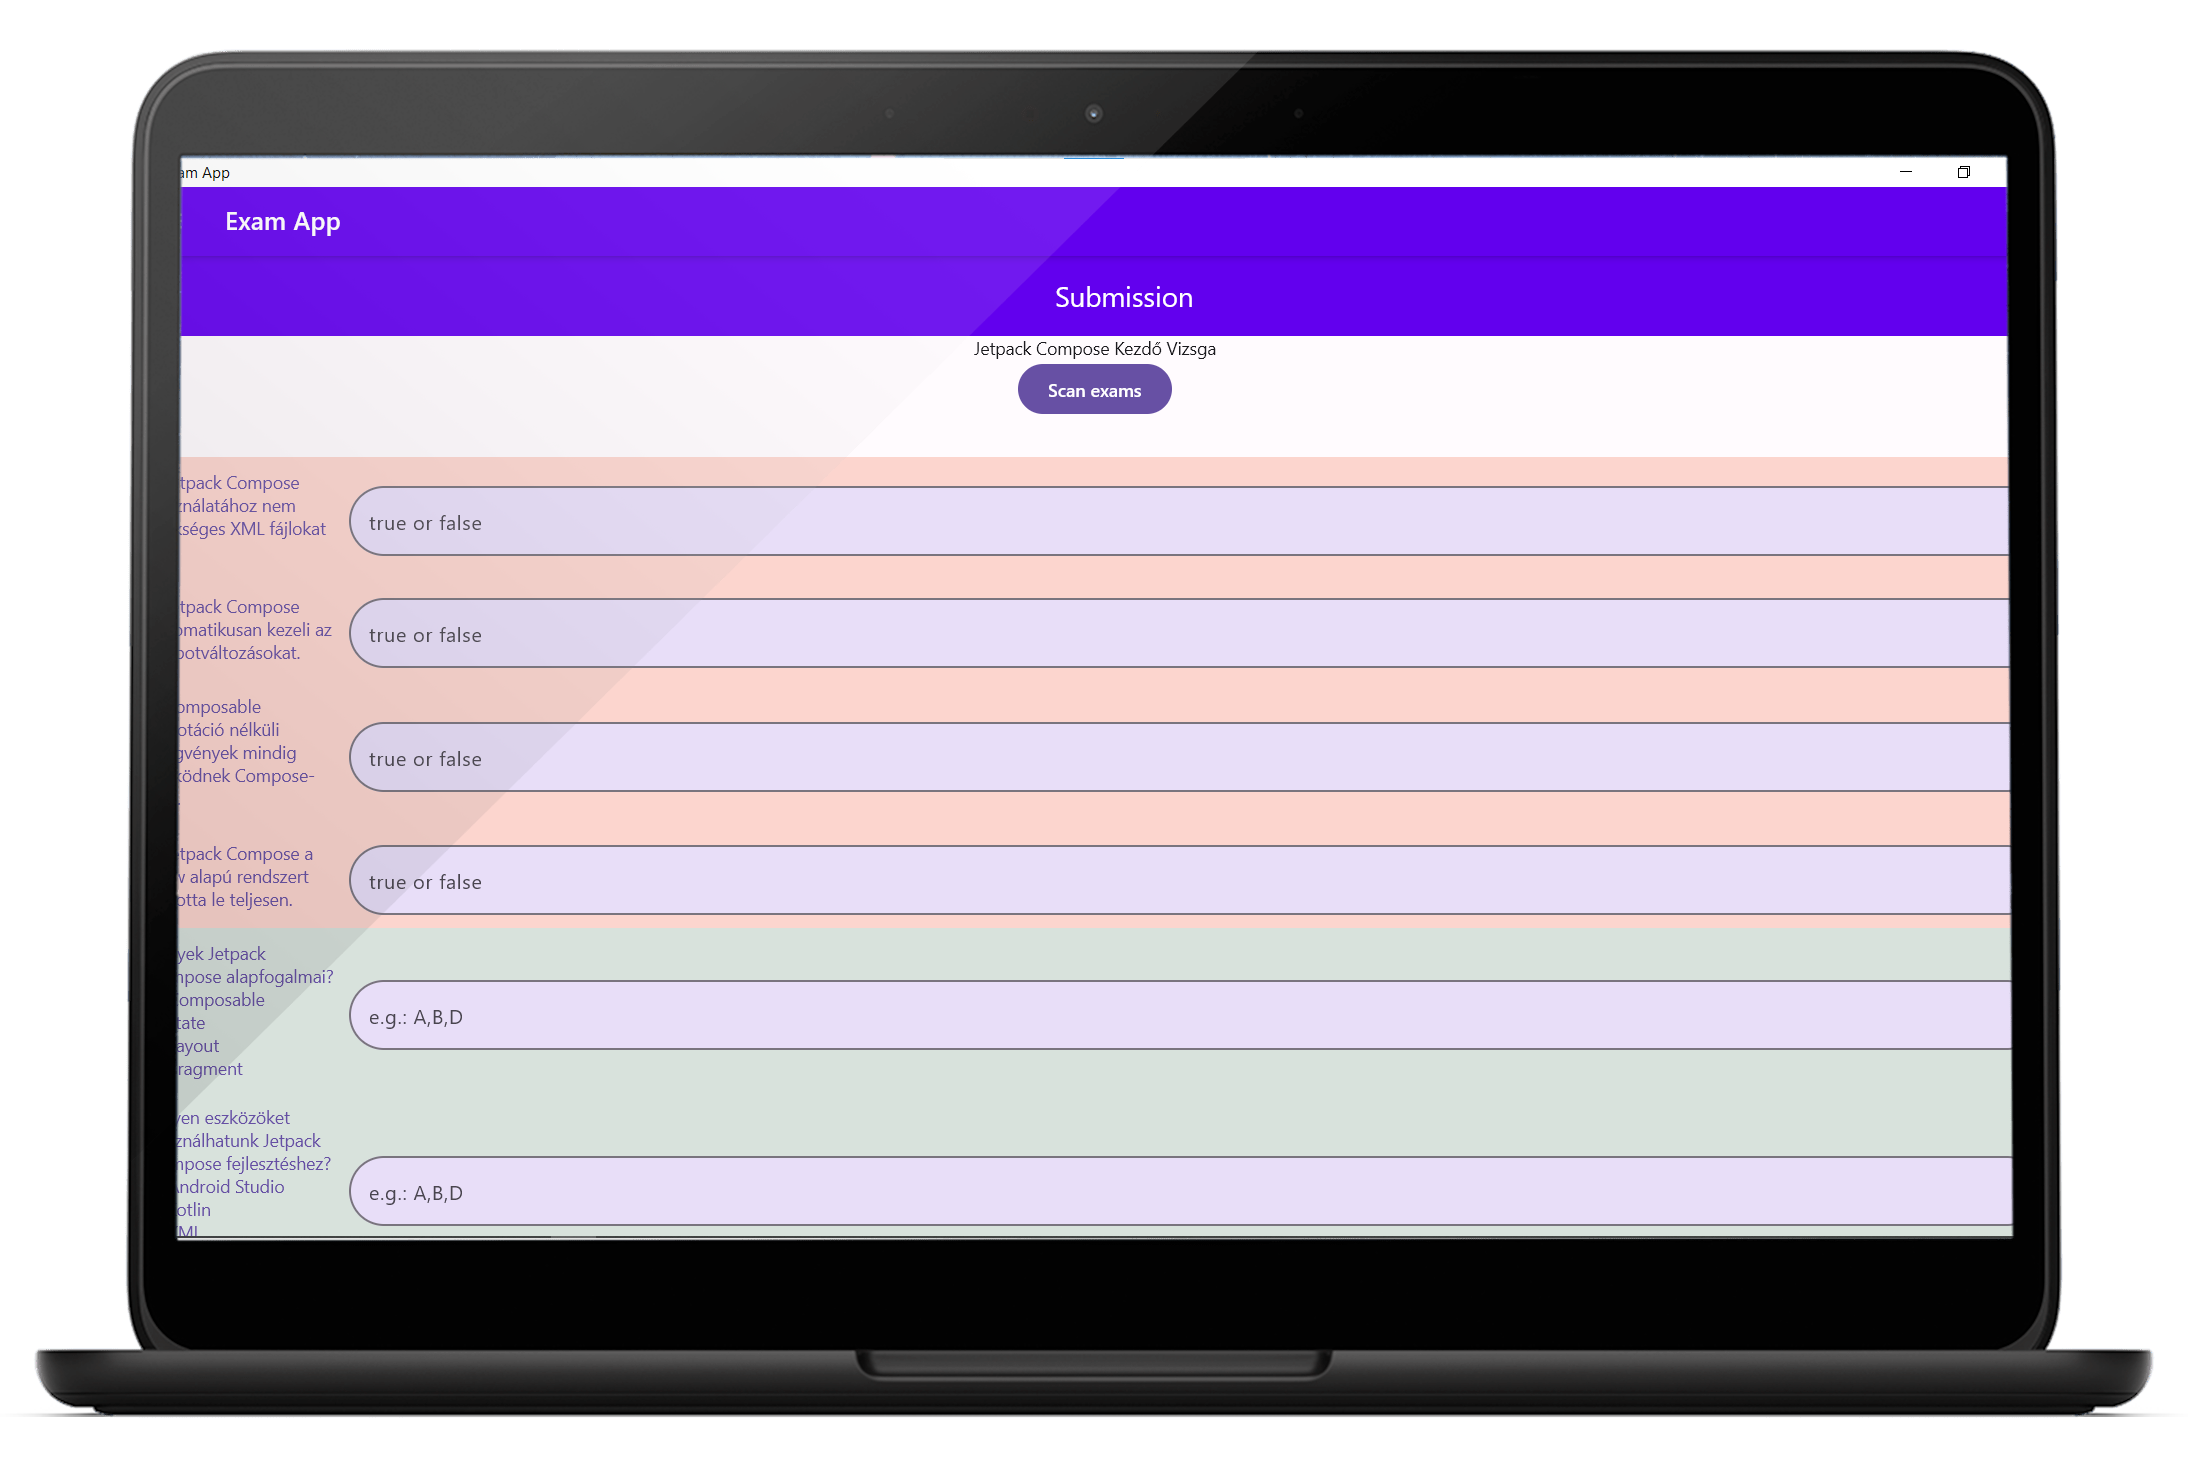
\includegraphics[width=0.6\textwidth, keepaspectratio]{figures/Submission_Desktop_framed.png}
    \end{tabular}
    \caption{Új feleletválasztós kérdés létrehozása.}
    \label{fig:SubmissionScreen}
\end{figure}


\subsection{Szekevencia diagram egy átlagos interakcióra}

Végezetül szeretnék bemutatni egy szekevencia diagramot amin keresztül mégerthető, hogy a felhasználó, az alkalmazás és a háttérben futó szerver milyen kapcsolatbanállnak egymással.

\begin{figure}[!ht]
    \centering
    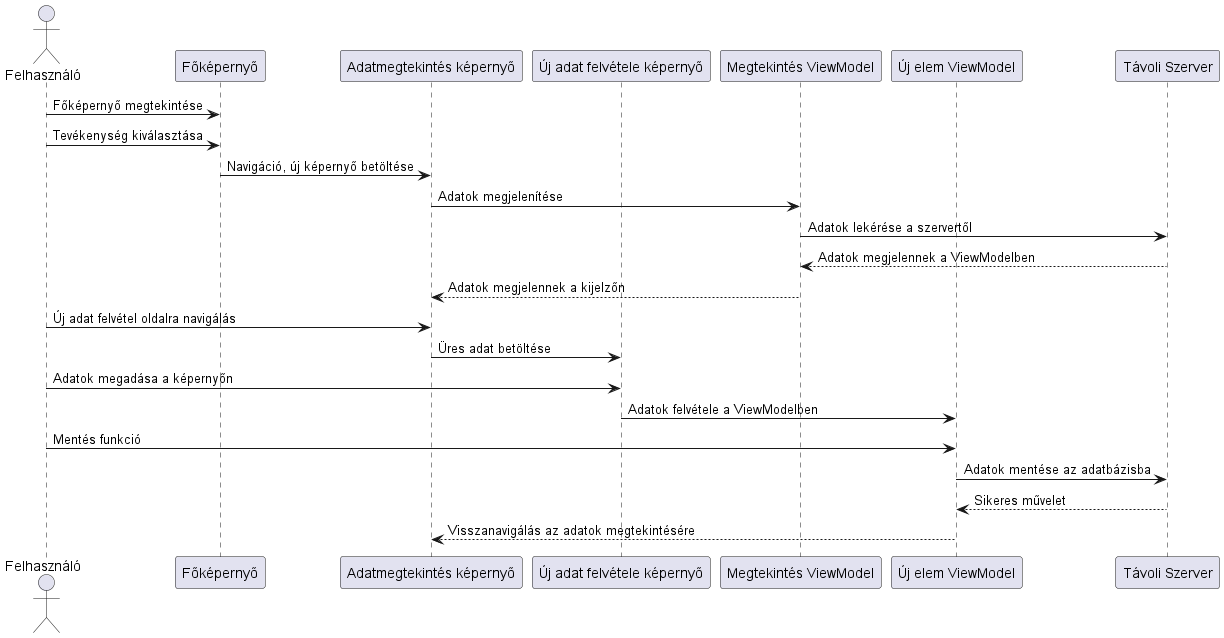
\includegraphics[width=150mm, keepaspectratio]{figures/Defaut Communication.png}
    \caption{Szekvencia diagram az end-to-end kommunikációról}
    \label{fig:DefaultCommunication}
\end{figure}

\section{Navigáció}
\label{sec:Nav}

A szoftverben az Androidból jól ismert navigációs könyvtárat használtam.
Szerencsére már jól integrálható multiplatform környezetben.
A \refstruc{sec:Navigation}ban erről már felületesen bemutattam.
Az ebben a fejezetben bemutatott implementációs lépéseket most részletesebben bemutatom.

Az első lépés kifejezetten egyszerű.
Létre kell hozni egy a végpontokat összefogó sealed classt, érdemes ennek egy route String típusú változót.
Ezt leginkább a böngészőben is megjelenő routinghoz hasonlít.
A sealed classból leszármaztathatunk data objeceteket. Ez egy viszonlylag egyedi felhasználás.
Itt az object egy singleton minta, mivel ebből az osztályból egy keletekezk összesen a program futása során.
A data keyword pedig létrehoz hasznos metódusokat az adateléréshez.
Tudunk megadni a leszármaztatott osztáylokban egyéb paramétereket így például tudunk egyes elemekre kulcsot adni amit ennek felhasználásával tudjuk a konrét példányt lekérdeni az adatbázsiból.

\begin{lstlisting}[caption={Példa a végpontok felvételére.}, label={lst:NavDestExample}, language=Kotlin]
sealed class ExamDestination(val route: String) {
    data object LoginScreenDestination : ExamDestination("LoginScreen")

    data object TopicDetailsDestination : ExamDestination("TopicDetails") {
    const val topicIdArg = "0"
    val routeWithArgs = "$route/{$topicIdArg}"
    }
}        
\end{lstlisting}

A másoik lépésben a NavHostControllert kell létrehozni. Ezt a rememberNavController() meghívásával tudjuk megtenni egy Composable függvény törzsén belül.
Ezt követően szükség lesz NavHost létrehozására ami egy Composablefüggvény.
Ennek lehet átadni az előbb létrehozott NavHostControllert, és be kell állítani egy kezeti végpontot ami az első composition során fog megjelenni.

A lenti példkódban látható az, hogy milyen módon lehet a NavHoston belül felevenni és használni a végpontokat.
Számos paraméter megadható, de ezek közül csak a route kötelező.
Megadahatók egyéb argumentumok, amiket az egyik képernyőről a másiknak szeretnénk átadani navArgumentek formájában.
Ezzel lehet például az egyedi azaonsírokat átadni a lista nézetről a részletes nézetnek.
Ezt követően az utolsó kötelező elem megadása a content, aminek a típusa: @Composable AnimatedContentScope.(NavBackStackEntry).
Ebből két dolog következik, ez egy Composable scope, így hívhatunk Composable függvényeket innen és, hogy hozzáférünk a BacstackEntryre tett adtaokat így például az argumentumokat.
Szintén ebben a lambda scopeban hozzáférünk a navControllerhez amivel a navigációt megvalüsító függvényeket tudjuk átadni a Viewnak.

\begin{lstlisting}[caption={Példa egy végpont felvételére a navigációs gráfban.}, label={lst:NavEndPointExample}, language=Kotlin]
composable(
    route = ExamDestination.TopicDetailsDestination.routeWithArgs,
    arguments = listOf(navArgument(ExamDestination.TopicDetailsDestination.topicIdArg) {
        type = NavType.StringType
    })
) {
    val id = it.arguments?.getString(ExamDestination.TopicDetailsDestination.topicIdArg) ?: "0"
    TopicDetailsScreen(
        navigateToEditTopic = { navController.navigate("${ExamDestination.TopicEditDestination.route}/$id") },
        topicId = id,
        navigateBack = { navController.popBackStack() }
    )
}    
\end{lstlisting}

A viewban, azaz a Composable függvényben a \ref{lst:NavEndPointExample}.~kódrészletben megírt függvényt tudjuk meghívni.

\begin{lstlisting}[caption={A navigáció viewban való megjelenése.}, label={lst:NavView}, language=Kotlin]
fun TopicDetailsScreenUiState(
    navigateToEditPoint: (String) -> Unit,
    navigateBack: () -> Unit,
    ...
){
    Scaffold(
        topBar = { TopAppBarContent(stringResource(Res.string.topic_details), navigateBack) },
        floatingActionButton = {
            FloatingActionButton(
                onClick = { navigateToEditPoint(topic.uuid) },
                shape = MaterialTheme.shapes.medium,
                modifier = Modifier.padding(20.dp)

            ) {...}
        }
    ) { ... }
}

\end{lstlisting}

\section{ViewModel}
\label{sec:VM}

A ViewModellel korábban a \refstruc{sec:ViewModel} és a \refstruc{sec:HighLevelArchitecture} részekben már foglalkoztam.
Ebben a részben egy megvalósításával fogok foglalkozni.

\begin{lstlisting}[caption={ViewModel implementációja.}, label={lst:VMImplementation}, language=Kotlin]
class TopicDetailsViewModel(
    var topicId: String,
) : ViewModel() {

    var topicDetailsScreenUiState: TopicDetailsScreenUiState by mutableStateOf(TopicDetailsScreenUiState.Loading)
    var uiState by mutableStateOf(TopicDetailsUiState())
    
    init { getTopic(topicId) }

    fun setId(id: String){ topicId = id; getTopic(id) }

    fun getTopic(topicId: String){
        topicDetailsScreenUiState = TopicDetailsScreenUiState.Loading
        viewModelScope.launch {
            topicDetailsScreenUiState = try{
                val result = ApiService.getTopic(topicId)
                uiState = TopicDetailsUiState(result.toTopicDetails(
                    parentName =
                    if (result.parentTopic == "null") ""
                    else ApiService.getTopic(result.parentTopic).topic
                ))
            TopicDetailsScreenUiState.Success(result)
            } catch (e: ApiException) {
                TopicDetailsScreenUiState.Error.errorMessage = e.message?: "Unkown error"
                TopicDetailsScreenUiState.Error
            }
        }
    }

    suspend fun deleteTopic() {
        try { ApiService.deleteTopic(topicId)} 
        catch (e: ApiException) {
            TopicDetailsScreenUiState.Error.errorMessage = e.message?: "Unkown error"
            topicDetailsScreenUiState = TopicDetailsScreenUiState.Error
        }
    }
}
\end{lstlisting}

A \ref{lst:VMImplementation}.~kódrészleten keresztül bemutatom a legfontosabb elemeket.
Az viewmdel osztály az általános Android ViewModel osztályból származik le.
Ez teszi lehetővé többek között a ViewModelScope használatát.
A szokásos módon adhatunk paramétereket, ebben az esetben így adjuk át az Id-t amivel a REST API-n keresztül tudjuk elérni a kívánt témakört.

Érdemes az osztály elején felvenni az állapotokat.
Ilyen Statekben tárolom a képernyő állapotát és a képernyőn megjelenő adatot is.
Ezeket a megfelelő kezdőértékkel létrehozva használhatjuk őket.
Lehetne MutabelStaeFlow is immutábilis Stateet használni egy másik megoldásként.

Az init{} blokk egyszer hívódik meg, az objektum létrehozása során a konstruktor után, ebből lehet több blokk is amik a leírt sorrendben hívódnak meg, későbbi init blokkban használhatjuk a korábbi értékekket.
Most itt egy aszinkron művelet eredményeként kapjuk meg az adatot.
Ezen kívül egy mésik inicailzációs elem a setId függvény, erre akkor van szükség amikor egy specifikus elemet akarunk megjeleníteni.

Az init{} blokkban nem tudunk tényleges aszinkron függvényeket hívni, ezért szükséges a töltőképernyő amíg az adatok megérkeznek.
A getTopic függvény kezeli le ezt a részt. Első lépés a töltőképernyő beállítsa. Ezt követően kihasználjuk a viwModelScopepot, ahol végrehajthatunk hosszabb műveletet anélkül, hogy a UI szál lefagyjon addig.
Itt megvárjuk amíg a REST API visszaküldi az adatokat, siker esetén a Succes képernyőt állítjuk be a stateben, hiba esetén erről adunk tájékoztatást.

Egyéb függvények megadhatók aszinkron módon, mint a törlés például, ezt nem kell megvárnunk.

\section{HTTP kliens}
\label{sec:HTTP}

Ebben a részben a HTTP kliens működését mutatom be.

\begin{lstlisting}[caption={HTTP kliens.}, label={lst:HTTPClient}, language=Kotlin]
object ApiService {
    private val httpClient = HttpClient() {
        install(ContentNegotiation) {
            json(Json {
                ignoreUnknownKeys = true
                prettyPrint = true
            })
        }
        defaultRequest { url("http://mlaci.sch.bme.hu:46258")  /* Set the base URL */ }
    }
    
    suspend fun getPoint(id: String): PointDto {
        val response = httpClient.get("/point/$id")
        if (response.status == HttpStatusCode.OK) return response.body()
        throw ApiException(handleHttpException(response.status))
    }

    suspend fun postPoint(point: PointDto): PointDto? {
        val response = httpClient.post("/point") {
            contentType(ContentType.Application.Json)
            setBody(point)
        }
        if (response.status == HttpStatusCode.Created) return response.body()
        throw ApiException(handleHttpException(response.status))
    }
}
\end{lstlisting}


A \ref{lst:HTTPClient}.~kódrészletben egy kis rész látható a komminikáció működéséről.
Egy objectben valósítom meg, így csak példány készül belőle.
Létrehozok benne egy HttpClientet aminek beállítom a tartalom típusát JSONre, és az alapértelmezett URL is beállításra kerül. 
Az endpontokban megadott részek ehhez lesznek hozzáfűzve így kevsebb kódot kell írnis kevesebb hibázási lehetőség van.

Ezek alatt aszinkron suspend függvények találhatóak. Mind a GET, POST, PUT és DELETE műveletkre vannak, de a GETen és a POSTon keresztül a lényeges részeket be lehet mutatni.
A függvények kaphatnak paramétereket, a GET esetén egy stringet ami a UUID értékét tartalmazza.
A visszatérési értéke pedig egy adott típusú dto lesz.
A kérést a baseURL + megadott útvonalra továbbítja a Ktor. Ezt a stinget lehet paraméterezni is, például az idval.
A válaszban megkapjuk a stászkódot és a válasz törzsében siker esetén a kért obkjektumot, amit a KotlinX szerilizáció állít elő a JSON adatból amit ténylgesen kapunk.
Hiba esetén a felhasználónak adunk erről visszajelzést egy saját kivételosztály segítségéve, 200 OK válasz esetánpedig átadjuk az elkészült adatot.
A listázós és a törlés ehhez hasonlómódon történik.

Az alsó függvény az új adat létrehozását mutatja be, lényegében a módosítás is szinte pont így történik, csak ott a PUT metódost kell hívni és a Created státszkódot várjuk helyes visszatérés esetén.
Itt paraméternek az objektumot kapjuk, amit a post üzenet törzsében állítunk be, itt történik meg a JSON szerilizáció, de most se kellezzel foglalkozni külön elég, ha az adat típusát megadjuk.
Innentől minden ugyan úgy történik, mint a többi esetben.


\section{PDF exportáló funkció}
\label{sec:PDF}

A feladatsor PDFbe exportálása más módon zajik a két platformon. 
Alapvetően hasinlüanműködnek.
Be kell állítani a megfelelő betűtípusokat, oldalméreteket, szövegméretet és hasonló egyéb változókat.

Ezt követően float értékek segítségével lehet pozícionálni a kiírandó szövegeket.
Táblázatokat nem lehet rajzolni, de egyéb geometriai elemekt, így vonalat igen, ezekből elkészíthető egy táblázat is.
Csak alacsony szintű támogatása van az APIknak, így ugyan minden elkészíthető, de nagyon időigényes.
Ahhoz, hogy egy jól kinéző dokumentum készüljön nagyon sok időt kell beletenni a megvalsításba.
PDF szerkesztésére és létrehozására így tehát nem ezek a legtökéletesebb megoldások.

\section{Szöveg felismerés}
\label{sec:TextRec}

A Szövegfelismeréshez a Google ML-Kit megoldását választttam.
Sok előre elkészített egyszerű AI modellt tartalmaz amit könynen lehet a kódban hasznosítani.
A használatát a \ref{lst:TextRec}.~kódrészlet mutatja be. 
A teljes kód látható egyben, mivel tömören és hatékonyan megoldható a probléma.
Ez a funkció Android eszözökön támogatott, asztali eszözökön nagyon furcsa lenne a használata.

Az osztály leszármazik a ImageAnalysis.Analyzer, így lehet képeket feldolgozó kódot létrehozni.
Be kell állítani az alapártékeket amikkel majd tud dolgozni az AI.
Ezt követőenmeg kell írni az egyetlen függvényt amit overrideolni kell, itt tötténik a kép feldolgozása, paramétere egy ImageProxy.
A szükséges hibakezelés után egy háttérszálon végrehjtódik a szöveg megkersése és felismerése a képen.
A szöveget ezt követően átadja a kód egy másik függvények, amit paraméterben adtunk meg, így tudjuk kinyerni az értékes adatokat.
Ez a kód amíg az adott nézeten vagyunk végtelen ideig fut, ezért szükség van egy kis késleltetésre, ezzel elkerülve a feleslges hardver használatot.

\begin{lstlisting}[caption={Szövegfelismerés.}, label={lst:TextRec}, language=Kotlin]
actual class TextRecognitionAnalyzer actual constructor(
    private val onDetectedTextUpdated: (String) -> Unit
) : ImageAnalysis.Analyzer {

    actual companion object {
        const val THROTTLE_TIMEOUT_MS = 1_000L
    }

    private val scope: CoroutineScope = CoroutineScope(Dispatchers.IO + SupervisorJob())
    private val textRecognizer: TextRecognizer =
        TextRecognition.getClient(TextRecognizerOptions.DEFAULT_OPTIONS)

    @OptIn(ExperimentalGetImage::class)
    override fun analyze(imageProxy: ImageProxy) {
        scope.launch {
            val mediaImage: Image = imageProxy.image ?: run { imageProxy.close(); return@launch }
            val inputImage: InputImage =
                InputImage.fromMediaImage(mediaImage, imageProxy.imageInfo.rotationDegrees)

            suspendCoroutine { continuation ->
                textRecognizer.process(inputImage)
                    .addOnSuccessListener { visionText: Text ->
                        val detectedText: String = visionText.text
                        if (detectedText.isNotBlank()) {
                            onDetectedTextUpdated(detectedText)
                        }
                    }
                    .addOnCompleteListener {
                        continuation.resume(Unit)
                    }
            }

            delay(THROTTLE_TIMEOUT_MS)
        }.invokeOnCompletion { exception ->
            exception?.printStackTrace()
            imageProxy.close()
        }
    }
}
\end{lstlisting}